\documentclass{ieeeaccess}

\usepackage{cite}
\usepackage{amsmath,amssymb}
\usepackage{graphicx}
\usepackage{textcomp}
\usepackage{booktabs}
\usepackage{array}
\usepackage{multirow}
\usepackage{url}

\usepackage{bm}
\makeatletter
\AtBeginDocument{\DeclareMathVersion{bold}
\SetSymbolFont{operators}{bold}{T1}{times}{b}{n}
\SetSymbolFont{NewLetters}{bold}{T1}{times}{b}{it}
\SetMathAlphabet{\mathrm}{bold}{T1}{times}{b}{n}
\SetMathAlphabet{\mathit}{bold}{T1}{times}{b}{it}
\SetMathAlphabet{\mathbf}{bold}{T1}{times}{b}{n}
\SetMathAlphabet{\mathtt}{bold}{OT1}{pcr}{b}{n}
\SetSymbolFont{symbols}{bold}{OMS}{cmsy}{b}{n}
\renewcommand\boldmath{\@nomath\boldmath\mathversion{bold}}}
\makeatother

\def\BibTeX{{\rm B\kern-.05em{\sc i\kern-.025em b}\kern-.08em
    T\kern-.1667em\lower.7ex\hbox{E}\kern-.125emX}}

\graphicspath{{raw_data/raw_data/}{figures/}}

\begin{document}
\raggedbottom
\history{Date of publication xxxx 00, 0000, date of current version xxxx 00, 0000.}
\doi{10.1109/ACCESS.2024.0429000}

\title{A Residual Decomposition Framework with Attention-Based Sequence Modeling for Renewable Energy Forecasting and Blockchain-Anchored Scheduling}

\author{\uppercase{Ankit Subedi}\authorrefmark{1},
\uppercase{Deepika J}\authorrefmark{1},
\uppercase{Abhishek Kumar}\authorrefmark{2}, AND
\uppercase{Liz Alex}\authorrefmark{1}}

\address[1]{Department of Information Security/CSE, School of Computer Science and Engineering, VIT University, Vellore, Tamil Nadu, India}
\address[2]{Department of Information Technology, School of Computer Science Engineering and Information Systems, VIT University, Vellore, Tamil Nadu, India}

\corresp{Corresponding author: Deepika J (e-mail: deepika.j@vit.ac.in).}

\markboth
{Subedi \headeretal: A Residual Decomposition Framework with Attention-Based Sequence Modeling}
{Subedi \headeretal: A Residual Decomposition Framework with Attention-Based Sequence Modeling}

\begin{abstract}
Accurate short-term renewable-energy forecasting is important for smart-grid operation because dispatch, storage, and renewable-aware scheduling decisions are sensitive to forecast error during high-variability periods. This paper presents a residual decomposition framework in which a multivariate Linear Regression (LR) model captures the dominant deterministic structure of hourly renewable generation, while a lightweight attention-based Bidirectional Long Short-Term Memory (BiLSTM) model is trained only on the residual error left by the linear component. The implementation uses 8760 hourly records derived from GridPath India renewable-resource data for Tamil Nadu, including fixed-tilt solar, single-axis solar, rooftop solar, adjusted onshore wind, engineered load, and storage-state features. A 48-hour lookback window with 10 input channels is used for sequence modeling. Evaluation across five random seeds shows that LR remains a very strong global baseline: LR obtains RMSE 0.006333, MAE 0.004678, and $R^2=0.988452$, while the Hybrid Residual model obtains RMSE $0.007187 \pm 0.001904$, MAE $0.005156 \pm 0.001064$, and $R^2=0.984295 \pm 0.009279$. A Diebold-Mariano test does not show statistically significant improvement of the Hybrid Residual model over LR on the full test set or on the peak subset where $y \ge 0.20$ (114 of 1266 test points). The contribution of the residual architecture is therefore framed as interpretability, failure-mode analysis, and deployable decomposition rather than as a global accuracy win over LR. Relative to Random Forest, the Hybrid Residual model reduces RMSE by 15.4\% and unexplained variance by 24.0\%. The blockchain component is presented as a prototype oracle architecture evaluated on a local Hardhat Ethereum node; a 12-module testing suite (62 test cases, all passing) validates hash integrity, chain linkage, PGS gating correctness, gas economics, pipeline latency (2.47~ms end-to-end), throughput (709 TPS for forecast anchoring), and storage efficiency (2.24:1 compression ratio). Privacy analysis and mainnet deployment remain future work. Under the same scheduling threshold of 0.15, LR and the Hybrid Residual model identify the same 280 eligible hours out of 1266 test hours and produce the same scheduled renewable share of 25.81\%, increasing renewable utilization from 15.34\% to 25.81\% during scheduled windows.
\end{abstract}

\begin{keywords}
Attention mechanism, bidirectional LSTM, blockchain oracle, energy-aware scheduling, residual decomposition, renewable-energy forecasting, smart grid.
\end{keywords}

\titlepgskip=-21pt

\maketitle

\section{Introduction}
Renewable energy forecasting is now a core requirement for power-system operation because solar and wind production varies with weather, time of day, and season. As renewable penetration increases, grid operators must make dispatch, storage, and scheduling decisions under greater uncertainty. Forecast error during peak-generation or transition periods can lead to underutilized renewable energy, unnecessary curtailment, increased reserve requirements, and inefficient downstream decisions~\cite{kroposki,pinson,voyant,denholm,lund,hong}. These effects are especially important in smart-grid settings where energy-aware compute scheduling, peer-to-peer energy exchange, and distributed control depend on forecast signals that are both accurate and auditable.

This research develops a residual decomposition methodology for forecasting total renewable energy output. The forecasting problem is decomposed into two component parts. First, the model captures the major renewable energy generating trends using Linear Regression. Second, the residuals generated by the linear model are fed into a Bidirectional Long Short-Term Memory (BiLSTM) network that focuses solely on predicting remaining nonlinear patterns. The residual error is defined as:
\begin{equation}
e_t = y_t - \hat{y}^{LR}_t .
\end{equation}
The final prediction is:
\begin{equation}
\hat{y}^{Hybrid}_t = \hat{y}^{LR}_t + \hat{e}^{BiLSTM}_t .
\end{equation}

The BiLSTM residual learner operates on a 48-hour lookback window with 10 input channels. By limiting its scope to analyzing the residual sequence rather than the full target, the recurrent network becomes smaller and easier to train compared to standalone deep-learning alternatives. Additionally, the use of attention weights allows the network to prioritize which hourly values are most relevant for correcting the linear forecast.

After each hour's value has been predicted, the model produces a Predictive Green Score (PGS). The PGS is a deterministic forecast-strength score defined as:
\begin{equation}
PGS_t = \operatorname{round}\left(10000 \cdot \operatorname{clip}(\hat{y}_t,0,1)\right),
\end{equation}
where $\hat{y}_t$ is the normalized forecast. The scheduling gate is:
\begin{equation}
E_t = \mathbb{1}[\hat{y}_t \ge 0.15] = \mathbb{1}[PGS_t \ge 1500].
\end{equation}
This is a deterministic forecast-strength score, not a calibrated probabilistic confidence score. Calibrated uncertainty-aware PGS design remains future work.

To support trustworthiness within multi-party environments, the forecasting model is integrated with a proposed oracle-style blockchain layer. The oracle layer records forecast payloads in canonical JSON format and anchors their digital fingerprints onto the blockchain. The validated forecasts are then available as inputs for renewable-aware scheduling and trading decisions. The pipeline is: ML Forecast $\rightarrow$ Canonical JSON $\rightarrow$ IPFS CID $\rightarrow$ Hash Anchor $\rightarrow$ Blockchain Validation $\rightarrow$ Trading/Scheduling. The blockchain component is explicitly scoped as a proposed architecture; no production smart-contract deployment, gas-cost benchmark, consensus-latency benchmark, privacy analysis, or adversarial security evaluation is claimed.

Overall, this research contributes to the following areas:
\begin{enumerate}
\item A residual decomposition framework for renewable energy forecasting that separates deterministic structure from stochastic deviations, enhancing model interpretability and learning efficiency.
\item A lightweight attention-based BiLSTM architecture operating on residual error to enable focused learning of nonlinearities and peak-hour anomalies.
\item A statistical robustness evaluation using peak-count reporting (114 of 1266 test points satisfy $y \ge 0.20$), Diebold-Mariano testing, and five random seeds.
\item A corrected scheduling interpretation that compares LR, Hybrid Residual forecasts, and perfect foresight under the same threshold rule.
\item A clarified blockchain-oracle formulation with an exact deterministic score definition (PGS) and an explicit boundary between proposed architecture and evaluated system behavior.
\end{enumerate}

Through empirical evaluations utilizing data derived from the GridPath India dataset for Tamil Nadu, this research demonstrates that scheduling renewables based upon forecasts can lead to significant increases in overall renewable utilization. Additionally, this research demonstrates that residual-learning achieves comparable performance to the strong linear baseline while providing an interpretable, decomposed architecture suitable for downstream control applications.


\section{Literature Review}
\subsection{Renewable Energy Forecasting}
Renewable energy forecasting has been studied using statistical, physical, machine-learning, and deep-learning approaches~\cite{voyant,inman,antonanzas,diagne,sobri,foley,hahn,wang_bilstm_access,dl_timeseries_access}. Classical time-series methods such as ARIMA and SARIMA provide interpretable temporal baselines and remain useful when seasonality is stable~\cite{box,hyndman}. However, renewable generation is affected by nonlinear interactions between irradiance, wind speed, installed capacity, and operational constraints. Machine-learning methods therefore became popular because they can map nonlinear feature interactions without requiring a full physical model~\cite{ahmad,mellit,jung}.

\subsection{Classical Machine-Learning Models}
Linear Regression is often competitive in structured energy datasets because generation profiles contain strong deterministic patterns from diurnal cycles and installed-capacity effects. Random Forest, extremely randomized trees, and gradient-boosted methods can capture nonlinear relationships and feature interactions~\cite{breiman,geurts,friedman,chen,ke}, but they do not directly model temporal sequence order unless lagged features are manually encoded. In the present work, both Linear Regression and Random Forest are used as baselines, while the Hybrid Residual model uses the linear component as a deterministic anchor rather than treating it only as a competitor.

\subsection{Recurrent Sequence Models}
The long short-term memory (LSTM) network was developed to deal with the issue of vanishing gradients in recurrent models~\cite{hochreiter}. Gated recurrent units, encoder-decoder sequence models, and probabilistic recurrent forecasters extended the application of deep sequence models for predicting time series~\cite{cho,sutskever,salinas}. Bidirectional recurrent networks process a sequence in both forward and backward directions to create richer contextual representations over the input window~\cite{schuster}. In forecasting, BiLSTM models can utilize the temporal context from windows of historical measurements. However, a standalone recurrent learner could be inefficient when the target includes a large deterministic portion. The recurrent model would need to learn both the smooth diurnal pattern and the irregular weather-driven deviation simultaneously. Residual learning overcomes this issue by requiring the sequence model to focus solely on learning the deviations about a strong baseline~\cite{he,oreshkin,lai,chen_residual_access}.

\subsection{Attention and Transformer-Based Models}
Attention mechanisms are capable of weighting different temporal positions in relation to how relevant they are to the task being modeled~\cite{bahdanau,luong}. The transformer architecture expands upon this concept via self-attention and has resulted in many successful applications within sequence modeling~\cite{vaswani}. Variants including temporal fusion transformer, informer, autoformer, FEDformer, PatchTST, and TimesNet have improved multi-horizon forecasting and long-sequence modeling~\cite{lim,zhou_informer,wu_autoformer,zhou_fedformer,nie,wu_timesnet}. However, traditional transformer architectures require quadratic memory growth with increasing sequence lengths and generally require larger training sets. Given moderately sized datasets and real-time deployment scenarios, lightweight attention-based recurrent models may serve as a more practical approach~\cite{li_attention_access,gao_attention_access,zhou_wind_bilstm_access}. Preliminary experiments conducted on the Tamil Nadu task demonstrated that multiple energy-aware attention variants produced minor marginal improvement before reaching a plateau. Due to these findings, the decision was made to pursue a residual decomposition strategy.

\subsection{Blockchain-Based Energy Systems}
The use of blockchain technology has received significant attention in terms of Transactive Energy, Peer-to-Peer Markets, Smart Contracts, and Decentralized Settlement~\cite{andoni,mengelkamp,aitzhan,li_consortium,kang,noor,mollah,szabo,buterin,tushar_access,wang_blockchain_access}, all of which enhance system-wide transparency. Most, however, rely upon historical meter reads or ex-post transactional logs. Trustworthy oracle mechanisms, decentralized data feeds, and authenticated off-chain computation are important considerations for blockchains that rely on physical world measurements or machine-learning predictions~\cite{albreiki,chainlink,zhang_towncrier,kosba,taghavi}.

\subsection{Research Gaps and Problem Formulation}
Three coupled gaps exist among the reviewed literature that motivate this study. First, although prior renewable forecasting studies have treated the full generation signal as a singular target for nonlinear models, this forces those same models to re-learn deterministic diurnal structures that simpler baselines already effectively capture; this waste of model capacity reduces robustness in high-variability environments. Second, there is little documentation of failure modes among prior evaluations of deep learning for energy forecasting. When standalone recurrent models perform worse than linear baselines, there is rarely documented evidence on why this occurred or what architectural modifications were attempted; thus practitioners lack actionable knowledge. Third, blockchain-based energy platforms and forecasting research are largely independent of one another; energy trading systems document transactions but do not document verifiable forecasts, whereas forecasting studies document accuracy metrics but do not provide an auditable means of enforcing signals for scheduling and trading purposes. There is no currently available integrated framework that serializes ML forecast payload outputs into distributed storage systems and utilizes them as on-chain gate logic for determining trading decisions. The Hybrid Residual model with blockchain oracle integration provides solutions for each of these three gaps. The above gaps are summarized in Table~\ref{tab:gaps}.

\begin{table*}[!t]
\caption{Comparison of Existing Models and Research Gaps}
\label{tab:gaps}
\centering
\begin{tabular}{p{2.8cm}p{3.2cm}p{3.2cm}p{3.2cm}p{3.2cm}}
\toprule
\textbf{Model / Approach} & \textbf{Key Strength} & \textbf{Limitation} & \textbf{Gap Identified} & \textbf{Proposed Advantage} \\
\midrule
Linear Regression (LR) & Simple, interpretable, strong for structured deterministic data & Cannot capture nonlinear and peak variations & Poor behavior in critical nonlinear regions & Residual learning models nonlinear deviations separately \\
\addlinespace
Random Forest (RF) & Captures nonlinear relationships and feature interactions & Lacks explicit temporal sequence modeling & Ignores ordered dependencies in energy data & BiLSTM captures temporal dynamics effectively \\
\addlinespace
LSTM & Models temporal dependencies through gated recurrence & Learns the full signal; may spend capacity on deterministic structure & Overburdened by deterministic and stochastic components & Residual decomposition reduces learning complexity \\
\addlinespace
BiLSTM & Captures bidirectional temporal context & Still processes the full target uniformly when used alone & Limited focus on high-impact deviations & Attention emphasizes influential residual windows \\
\addlinespace
Transformer & Powerful self-attention and parallel processing & Higher computational cost and data demand & Less suitable for moderate datasets and edge use & Lightweight attention-BiLSTM provides efficient alternative \\
\addlinespace
Blockchain Energy Systems & Transparency, decentralization, and auditable settlement & Often depend on historical or static data & Forecast signals are not integrated as verifiable control inputs & Oracle-based anchoring enables trusted forecast-driven decisions \\
\bottomrule
\end{tabular}
\end{table*}


\section{System Overview}
\subsection{Integrated Forecasting and Decision Architecture}
The proposed integrated framework links forecasting, validation, and scheduling within one decision pathway. Renewable data from Tamil Nadu is used to create both cyclical and physical features from modeled and observed operating data. The residual structure learned by the attention-based BiLSTM model plus a linear baseline represents the dominant deterministic relationship. The corrected forecast along with metadata is then forwarded to an oracle layer for validation and anchoring prior to being consumed by scheduling or trading logic. The key architectural contribution is that these three layers (forecasting, blockchain decision, and actuation) were developed together. Forecasting is not treated as a secondary product; rather, it is the primary operational variable determining if trading or energy-intensive execution should occur.

\subsection{Blockchain as Decision-Layer Infrastructure}
In the design of this integrated framework, blockchain is utilized as the decision-layer infrastructure due to its ability to provide trust, transparency, and tamper-proof validation in multi-party energy systems~\cite{blockchain_dispatch_access}. Through cryptographic hashing and distributed-consensus mechanisms, this system provides assurance that forecast-driven scheduling and trading decisions are auditable and cannot be manipulated by any actor. This is particularly important in peer-to-peer energy networks and renewable-aware compute-scheduling environments where numerous actors need to operate under shared forecast signals.

The mechanism of integration is as follows: after forecasting has occurred, a validation node bundles the forecasted value along with relevant feature attributes, timestamp, and schedule-eligibility metadata into a canonical JSON object. It is crucial to serialize this object deterministically because standard JSON objects may vary by key ordering and whitespace. Once serialized, the payload is written off-chain to the Interplanetary File System (IPFS), which returns a Content Identifier (CID)~\cite{ipfs_blockchain_access}. At the same time, the payload is hashed using keccak256 and only the compact fingerprint along with the CID and associated renewable score are stored on-chain to prevent blockchain bloat while maintaining full verifiability.

The oracle layer performs four functions: (1) validates the forecast payload and metadata; (2) calculates a cryptographic digest of the forecast object; (3) anchors the digest to a ledger record via consensus; and (4) exposes the validated forecast as an input to decision-layer scheduling and trading logic.

\textbf{Scope clarification:} The blockchain component includes a working Solidity prototype evaluated on a local Hardhat Ethereum node with measured gas costs, latency, throughput, and a 12-module automated testing suite (Section VII). Privacy analysis and mainnet deployment remain future work.


\section{Methodology}
\subsection{Problem Formulation}
Let $\mathbf{x}_t$ denote the multivariate feature vector at time $t$, including renewable capacity factors, generated power, modeled load, modeled state of charge, and cyclical time encodings. The target $y_t$ is the normalized renewable-generation signal in log-transformed form:
\begin{equation}
y_t = \log\left(1 + \frac{P^{gen}_t}{P^{peak}}\right),
\end{equation}
where $P^{gen}_t$ is total renewable generation and $P^{peak}$ is the peak-load normalization constant. The model uses $\mathbf{X}_{t-L+1:t}$ with a lookback window $L=48$ hours. The main challenge is that the series contains both linear and nonlinear components. The majority of the series is a function of time with strong periodic nature due to solar position and wind patterns. However, some portions reflect abrupt changes due to localized weather conditions or variations in storage load, which are operationally significant.

\subsection{Dataset Construction}
The core renewable generation data is derived from the GridPath India long-term power-system planning dataset, which provides hourly capacity-factor traces for solar and wind resources~\cite{gridpath}. Tamil Nadu records are filtered from fixed-tilt solar PV, single-axis solar PV, rooftop solar PV, and adjusted existing wind folders. Each source is checked for hourly continuity, missing timestamps, duplicate timestamps, and null values. The final hourly renewable table contains 8760 observations for calendar year 2019.

Modeled load is represented with a deterministic daily profile bounded between 7000~MW and 14000~MW. Modeled battery state of charge (SoC) follows configured storage limits, charge/discharge efficiencies, and maximum rate constraints. These modeled components provide a consistent evaluation environment and do not replace the underlying real-world generation data.

\begin{table}[!t]
\caption{Dataset and Feature Summary}
\label{tab:dataset_summary}
\centering
\begin{tabular}{ll}
\toprule
Item & Description \\
\midrule
Temporal coverage & 8760 hourly observations (2019) \\
Region & Tamil Nadu, India \\
Renewable inputs & Fixed-tilt solar, single-axis solar, \\
 & rooftop solar, adjusted wind CFs \\
Modeled variables & Load demand, battery SoC \\
Target & $\log(1 + P^{gen}/P^{peak})$ \\
Feature set & Renewable factors, $P^{gen}$, $P^{load}$, \\
 & SoC, hour sin/cos, day sin/cos \\
\bottomrule
\end{tabular}
\end{table}

\subsection{Preprocessing Pipeline}
The preprocessing pipeline performs deterministic file discovery, schema validation, Tamil Nadu filtering, timestamp parsing, per-folder aggregation, and final merge. Capacity factors are averaged across Tamil Nadu projects at each timestamp. Cyclical features are encoded as:
\begin{equation}
h^{sin}_t = \sin\left(\frac{2\pi h_t}{24}\right), \quad h^{cos}_t = \cos\left(\frac{2\pi h_t}{24}\right),
\end{equation}
with analogous encodings for day of year. These encodings prevent artificial discontinuity between adjacent hours such as 23:00 and 00:00.

\subsection{Residual Decomposition Logic}
The residual decomposition first trains a Linear Regression model $f_{LR}$:
\begin{equation}
\hat{y}^{LR}_t = f_{LR}(\mathbf{X}_{t-L+1:t}).
\end{equation}
The residual target is then defined as:
\begin{equation}
r_t = y_t - \hat{y}^{LR}_t.
\end{equation}
The sequence model focuses solely on the stochastic errors. By removing much of the variation from the original target through reduction to a residual, the learning process becomes more efficient and stable. From exploratory analysis, 64 extremely nonlinear points out of 1266 test points (5.1\%) were identified, concentrated at high-generation periods and time transitions where operational cost of miscalculation is greatest. Linear Regression provided sufficient explanation for modeling base trends, and residual error analysis showed the remaining problem was smaller and more localized.

\subsection{Attention-Based BiLSTM Residual Learner}
The residual learner receives a 48-hour lookback sequence with 10 input channels. A bidirectional LSTM layer extracts temporal features from both forward and backward directions. The bidirectional structure is motivated by the observation that renewable generation is influenced not only by the most recent hours but also by where the current hour lies within the surrounding diurnal pattern. The attention scoring function computes a saliency score for each hidden state:
\begin{equation}
e_i = \tanh(\mathbf{W}_a\mathbf{h}_i + \mathbf{b}_a),
\end{equation}
which is normalized via softmax to produce attention weights and an attention-weighted context vector:
\begin{equation}
\alpha_i = \frac{\exp(e_i)}{\sum_{j=1}^{L}\exp(e_j)}, \quad \mathbf{c} = \sum_{i=1}^{L}\alpha_i\mathbf{h}_i,
\end{equation}
where $\mathbf{h}_i$ is the hidden state and $\mathbf{c}$ is the context vector. The context is projected to the residual estimate:
\begin{equation}
\hat{\varepsilon}_t = \mathbf{W}_o \cdot \varphi(\mathbf{W}_c\mathbf{c}_t + \mathbf{b}_c) + \mathbf{b}_o,
\end{equation}
where $\varphi$ denotes ReLU activation. Attention is included because not every hour contributes equally to the residual: peak-generation errors are often driven by the interaction between immediate short-horizon fluctuations and periodic diurnal recurrence.

\begin{table}[!t]
\caption{Attention-Based BiLSTM Residual Learner Architecture}
\label{tab:architecture}
\centering
\begin{tabular}{lcc}
\toprule
Layer & Output Shape & Parameters \\
\midrule
Input & (48, 10) & 0 \\
Bidirectional LSTM & (48, 32) & 3,456 \\
Attention layer & (32) & 80 \\
Dropout & (32) & 0 \\
Dense & (16) & 528 \\
Output dense & (1) & 17 \\
\midrule
\textbf{Total} & -- & \textbf{4,081} \\
\bottomrule
\end{tabular}
\end{table}

\subsection{Model Architecture}
Table~\ref{tab:architecture} reports the exact architecture. The model has 4,081 trainable parameters, making it substantially lighter than typical Transformer-based alternatives.

\subsection{BiLSTM Selection Rationale}
While Transformer-based architectures offer powerful sequence modeling capabilities through self-attention mechanisms, they typically require larger datasets and higher computational resources. Recent deep-learning surveys confirm that hybrid recurrent-attention architectures remain competitive for moderate-scale energy data~\cite{dl_timeseries_access,lee_solar_access,abdel_nabi_access}. The present dataset has 8760 hourly observations and 6084 training sequences after lookback construction. For this scale, a 4,081-parameter attention-BiLSTM is more efficient and easier to deploy near the edge than a full Transformer. The proposed Hybrid Residual model shares conceptual similarity with Transformer attention in its ability to emphasize salient temporal features; however, it retains a recurrent structure more suitable for moderate-sized datasets. In preliminary experimentation, GRU models were notably unstable and underperformed substantially, while plain LSTM models were more competitive but insufficient when trained end-to-end on the full target.

\subsection{Residual Learning Justification}
The choice of residual decomposition over full-signal learning rests on three complementary arguments. First, the Tamil Nadu generation signal is dominated by a near-deterministic diurnal and seasonal skeleton. Fitting a nonlinear model to this signal forces it to allocate most capacity to re-discovering structure that a linear model already captures with high fidelity. The residual has substantially lower variance than the original target, making the nonlinear learning problem more tractable and convergence more stable. Second, if either the additive noise branch or the attention-BiLSTM learns a nearly zero residual, the composite model behaves like the linear baseline rather than diverging. This provides a safe operating condition since forecasting errors in scheduling can lead to trading errors or unnecessary storage cycling. Third, EA-BiLSTM v1, v2, and ACHF were all trained end-to-end on the full normalized target despite increasing architectural complexity, and none outperformed Linear Regression on global error measures. By decomposing into a linearizable portion and training the residual using a significantly reduced sparse target, both issues were simultaneously addressed.


\section{Experimental Setup}
\subsection{Data Split and Sequence Construction}
The hourly dataset is split into train, validation, and test partitions with chronological order preserved. The raw split sizes are 6132 training observations, 1314 validation observations, and 1314 test observations. After applying a 48-hour lookback, the sequence tensors contain 6084 training sequences, 1266 validation sequences, and 1266 test sequences. The test interval spans November 9, 2019 06:00 through December 31, 2019 23:00. Continuous exogenous features are standardized using StandardScaler fit on the training partition only, then applied to validation and test partitions to avoid leakage.

\subsection{Baselines}
Two baseline models are used. Linear Regression is trained on flattened 48-hour sequence windows and represents the deterministic reference model. Random Forest is trained on the same flattened representation with 200 trees, maximum depth 12, and minimum leaf size 2, and represents a nonlinear non-sequential baseline. The proposed Hybrid Residual model uses the Linear Regression prediction as the deterministic component and the attention-BiLSTM output as the residual correction.

\subsection{Training Configuration}
The BiLSTM is trained with mean-squared error loss and MAE monitoring. Early stopping with restored best weights prevents unnecessary training once validation loss stops improving~\cite{prechelt}. Dropout regularization and adaptive optimization are used to stabilize training~\cite{kingma,srivastava}. A reduce-on-plateau schedule with factor 0.5, patience 5, and minimum learning rate $10^{-6}$ decreases the learning rate when validation loss stagnates. The implementation uses scikit-learn for classical baselines and TensorFlow/Keras for the neural residual learner~\cite{pedregosa,tensorflow,keras}.

\begin{table}[!t]
\caption{Training Configuration and Quantitative Justification}
\label{tab:training_config}
\centering
\begin{tabular}{lll}
\toprule
Parameter & Value & Justification \\
\midrule
Lookback window & 48 h & Two full diurnal cycles \\
BiLSTM units & 16/dir. & 4,081 params total \\
Dropout rate & 0.2 & Reduces overfitting \\
Batch size & 64 & Balances gradient noise \\
Initial LR & $10^{-3}$ & Adam default \\
Min. learning rate & $10^{-6}$ & Prevents excess reduction \\
Early-stop patience & 15 epochs & Best weights restored \\
Loss function & MSE & Standard for regression \\
Optimizer & Adam & Adaptive moment estimation \\
Validation metric & MAE & Robust to outlier residuals \\
Max epochs & 200 & Sufficient ceiling \\
Seeds & 42, 123, 456, & Five-seed robustness \\
 & 789, 2024 & \\
\bottomrule
\end{tabular}
\end{table}

\subsection{Standalone EA-BiLSTM Tuning Campaign}
Prior to adopting the residual decomposition strategy, three standalone energy-aware BiLSTM variants were systematically evaluated on the full normalized target, documenting both configuration and measured outcomes to justify the architectural pivot.

EA-BiLSTM v1 employed a standard bidirectional LSTM encoder with a single-head attention layer trained end-to-end on the full log-transformed target. Despite competitive early-training validation loss, the model failed to generalize on the test set, achieving test $R^2$ of 0.942 and test RMSE of 0.014145---substantially worse than the Linear Regression baseline (RMSE 0.006333).

EA-BiLSTM v2 introduced energy-weighted attention gating, assigning higher importance scores to time steps associated with elevated observed generation. This improved test $R^2$ to 0.933 and reduced test RMSE to 0.015304, but performance remained below both Linear Regression and Random Forest.

EA-BiLSTM ACHF (Adaptive Cross-Horizon Fusion) added a learnable fusion layer combining short-horizon and long-horizon hidden states. Despite additional parameters, this variant achieved test $R^2$ of 0.871 and RMSE of 0.021148---still inferior to Linear Regression on global RMSE. This confirmed that the task contains more linearizable structure than standalone BiLSTM elaboration can overcome.

\begin{table}[!t]
\caption{Standalone Sequence Model Results (Log-Scale)}
\label{tab:standalone}
\centering
\begin{tabular}{lccp{3.5cm}}
\toprule
Variant & Test $R^2$ & Test RMSE & Key Change \\
\midrule
LSTM & 0.942398 & 0.014145 & Standard LSTM; full-signal target \\
GRU & 0.932567 & 0.015304 & Gated recurrent unit \\
BiLSTM & 0.871241 & 0.021148 & Bidirectional; full-signal target \\
\textbf{Hybrid Residual} & \textbf{0.984295} & \textbf{0.007187} & Residual decomposition; BiLSTM on error only \\
\bottomrule
\end{tabular}
\end{table}


\section{Results and Evaluation}
\subsection{Global Forecasting Performance}
Table~\ref{tab:global_performance} reports validation and test metrics for all evaluated models. Linear Regression and the Hybrid Residual model show comparable global performance. Although the Hybrid Residual model achieves performance comparable to Linear Regression on global error metrics, its primary contribution is the decomposed, auditable architecture rather than a global accuracy win. The comparison with Linear Regression should be read as practical parity on global metrics. The Tamil Nadu series is sufficiently structured that a simple linear model already provides a very strong global baseline. Relative to Random Forest, the Hybrid Residual model reduces test RMSE by 18.6\% (from 0.008497 to 0.006918) and reduces unexplained variance by 33.7\%.

\begin{table}[!t]
\caption{Global Model Performance (Log-Scale, Unified Evaluation)}
\label{tab:global_performance}
\centering
\begin{tabular}{lccc}
\toprule
Model & Test RMSE & Test MAE & Test $R^2$ \\
\midrule
LSTM (standalone) & 0.014145 & 0.010960 & 0.942398 \\
GRU (standalone) & 0.015304 & 0.012187 & 0.932567 \\
BiLSTM (standalone) & 0.021148 & 0.016194 & 0.871241 \\
Linear Regression & 0.006333 & 0.004678 & 0.988452 \\
Random Forest & 0.008497 & 0.006007 & 0.979212 \\
Hybrid Residual (5-seed mean) & 0.007187 & 0.005156 & 0.984295 \\
Hybrid Residual (5-seed std.) & $\pm$0.001904 & $\pm$0.001064 & $\pm$0.009279 \\
\bottomrule
\end{tabular}
\end{table}

\subsection{Single-Run Metrics (Historical Reference)}
The earlier manuscript reported a single-run comparison in which LR and the Hybrid Residual model were nearly identical. That result is retained only as a historical single-run output, not as the final robustness claim.

\begin{table}[!t]
\caption{Historical Single-Run Metrics}
\label{tab:single_run}
\centering
\begin{tabular}{lccc}
\toprule
Model & Test RMSE & Test MAE & Test $R^2$ \\
\midrule
Linear Regression & 0.007334 & 0.005305 & 0.988058 \\
Hybrid Residual (single run) & 0.007337 & 0.005312 & 0.988051 \\
Random Forest & 0.009822 & 0.006824 & 0.978584 \\
\bottomrule
\end{tabular}
\end{table}

\subsection{Peak-Generation Subset}
Using $y \ge 0.20$, the peak subset contains 114 test points out of 1266, or 9.0\%. On this subset, LR and the Hybrid Residual model are near-tied.

\begin{table}[!t]
\caption{Peak-Subset Comparison ($y \ge 0.20$, $n=114$)}
\label{tab:peak_subset}
\centering
\begin{tabular}{lcc}
\toprule
Metric & Linear Regression & Hybrid Residual \\
\midrule
Peak RMSE & 0.009724 & 0.009738 \\
Peak MAE & 0.007502 & 0.007508 \\
RMSE difference & \multicolumn{2}{c}{$-0.14\%$} \\
MAE difference & \multicolumn{2}{c}{$-0.08\%$} \\
\bottomrule
\end{tabular}
\end{table}

\subsection{Diebold-Mariano Significance Test}
The Diebold-Mariano (DM) test compares predictive accuracy using loss differentials. Positive loss differential means the Hybrid Residual model is better. The test does not show significant improvement for the Hybrid Residual model on either the full-test or peak-test subset.

\begin{table}[!t]
\caption{Diebold-Mariano Test: LR vs.\ Hybrid Residual (Log-Scale)}
\label{tab:dm_test}
\centering
\begin{tabular}{lccc}
\toprule
Metric & Value & & \\
\midrule
Seeds with $p<0.05$ & 1 of 5 & & \\
Mean DM statistic & $-0.3858 \pm 1.7006$ & & \\
Mean DM $p$-value & 0.2022 & & \\
\bottomrule
\end{tabular}
\end{table}

The mean DM statistic of $-0.39$ with $p=0.20$ indicates that the difference between LR and the Hybrid Residual model is not statistically significant at $\alpha=0.05$. Only 1 of 5 seeds achieves significance, confirming near-parity.

\subsection{Repeated-Seed Robustness}
Table~\ref{tab:seed_results} summarizes five Hybrid Residual training runs. Only one seed produces a significant DM result at $p<0.05$, and the average DM statistic remains negative. The revised conclusion is that the Hybrid Residual model achieves near-parity but does not consistently outperform LR.

\begin{table}[!t]
\caption{Hybrid Residual Model Across Five Seeds (Log-Scale)}
\label{tab:seed_results}
\centering
\begin{tabular}{rccccc}
\toprule
Seed & RMSE & MAE & $R^2$ & Peak RMSE & DM $p$ \\
\midrule
42 & 0.006369 & 0.004711 & 0.988321 & 0.009732 & 0.4507 \\
123 & 0.006320 & 0.004668 & 0.988500 & 0.009732 & 0.3136 \\
456 & 0.010592 & 0.007060 & 0.967698 & 0.011546 & 0.1376 \\
789 & 0.006352 & 0.004696 & 0.988384 & 0.009719 & 0.0171 \\
2024 & 0.006300 & 0.004647 & 0.988574 & 0.009750 & 0.0918 \\
\bottomrule
\end{tabular}
\end{table}

\subsection{Prediction Tracking}
Predictive performance of the Hybrid Residual model and Linear Regression are compared for each time step. The predictions follow the general shape of the actual generation pattern well. Deviations mostly appear during transitions between consecutive days or at local maximum/minimum generation, supporting the decomposition concept: the global part can be modeled deterministically while the residual variation should be estimated based on past deviations.

\subsection{Error Distribution}
The error distribution of the Hybrid Residual model has mean error $-0.000404$ and standard deviation $0.007326$. The concentration of error around zero indicates little bias. However, the long tail indicates that some operating conditions contribute significantly to overall error---these represent conditions where forecasts are most likely to fail.

\subsection{Residual and Heteroscedastic Error Analysis}
Residuals of the linear baseline occur at specific times (not randomly distributed) as opposed to being uniformly distributed. A closer examination reveals heavy-tailed distributions, and residual spreads increase as actual generation increases---a classic sign of heteroscedastic behavior. When generation is low, the linear baseline follows the actual signal closely. When generation increases significantly, the residual fans out rapidly.

\subsection{Diagnostic Comparison by Generation Tier}
Table~\ref{tab:diagnostic_tier} presents global and peak-band RMSE. There is no substantial difference among the three models at lower generation levels; however, at higher generation levels, the differences become more relevant for operational decisions.

\begin{table}[!t]
\caption{Diagnostic Comparison by Generation Tier (Log-Scale)}
\label{tab:diagnostic_tier}
\centering
\begin{tabular}{lcc}
\toprule
Model & Global RMSE & Peak RMSE ($y_t \ge 0.20$) \\
\midrule
Linear Regression & 0.006333 & 0.009724 \\
Random Forest & 0.008497 & -- \\
Hybrid Residual (mean) & 0.007187 & 0.010096 \\
\bottomrule
\end{tabular}
\end{table}

\subsection{Ablation Study}
Two ablation studies analyze individual contributions. Table~\ref{tab:ablation_decomp} evaluates the decomposition principle. Removing residual decomposition and training the BiLSTM directly on the full target degrades test RMSE substantially. Keeping the linear baseline but replacing the BiLSTM residual learner with a mean residual predictor confirms that the BiLSTM contributes meaningful nonlinear correction beyond a trivial zero-residual fallback. The full two-stage architecture achieves the best balance of global accuracy and peak-period reliability.

\begin{table}[!t]
\caption{Decomposition Ablation: Effect of Residual Split (Log-Scale)}
\label{tab:ablation_decomp}
\centering
\begin{tabular}{lccc}
\toprule
Configuration & Test RMSE & Test MAE & Test $R^2$ \\
\midrule
BiLSTM full-target & 0.021148 & 0.016194 & 0.871241 \\
LR + mean residual & 0.006333 & 0.004678 & 0.988452 \\
LR + attn-BiLSTM (Hybrid Residual) & 0.007187 & 0.005156 & 0.984295 \\
\bottomrule
\end{tabular}
\end{table}

Table~\ref{tab:variant_ablation} illustrates the historical EA-BiLSTM progression, showing how the transition from standalone BiLSTM elaboration to residual decomposition provided the largest increase in performance.

\begin{table}[!t]
\caption{Historical Variant Ablation: EA-BiLSTM Progression (Log-Scale)}
\label{tab:variant_ablation}
\centering
\begin{tabular}{lccc}
\toprule
Variant & Test RMSE & Test MAE & Test $R^2$ \\
\midrule
LSTM (standalone) & 0.014145 & 0.010960 & 0.942398 \\
GRU (standalone) & 0.015304 & 0.012187 & 0.932567 \\
BiLSTM (standalone) & 0.021148 & 0.016194 & 0.871241 \\
\textbf{Hybrid Residual} & \textbf{0.007187} & \textbf{0.005156} & \textbf{0.984295} \\
\bottomrule
\end{tabular}
\end{table}

The visual progression reinforces the limitations of standalone architectures. While algorithmic modifications such as energy-weighted gating (v2) and architectural fusions (ACHF) drive consecutive improvements in MAE and $R^2$, the trajectory demonstrates diminishing returns. The standalone recurrent models struggle to implicitly encode the rigid daily and seasonal bounds of the grid schedule. By contrast, the abrupt improvement achieved by the proposed residual model validates the transition to a residual modeling approach. By delegating the mathematically simple, repetitive diurnal patterns to the Linear Regression baseline, the BiLSTM architecture immediately achieves superior generalization, operating purely as a specialized nonlinear corrector.

\begin{figure}[!t]
\centering
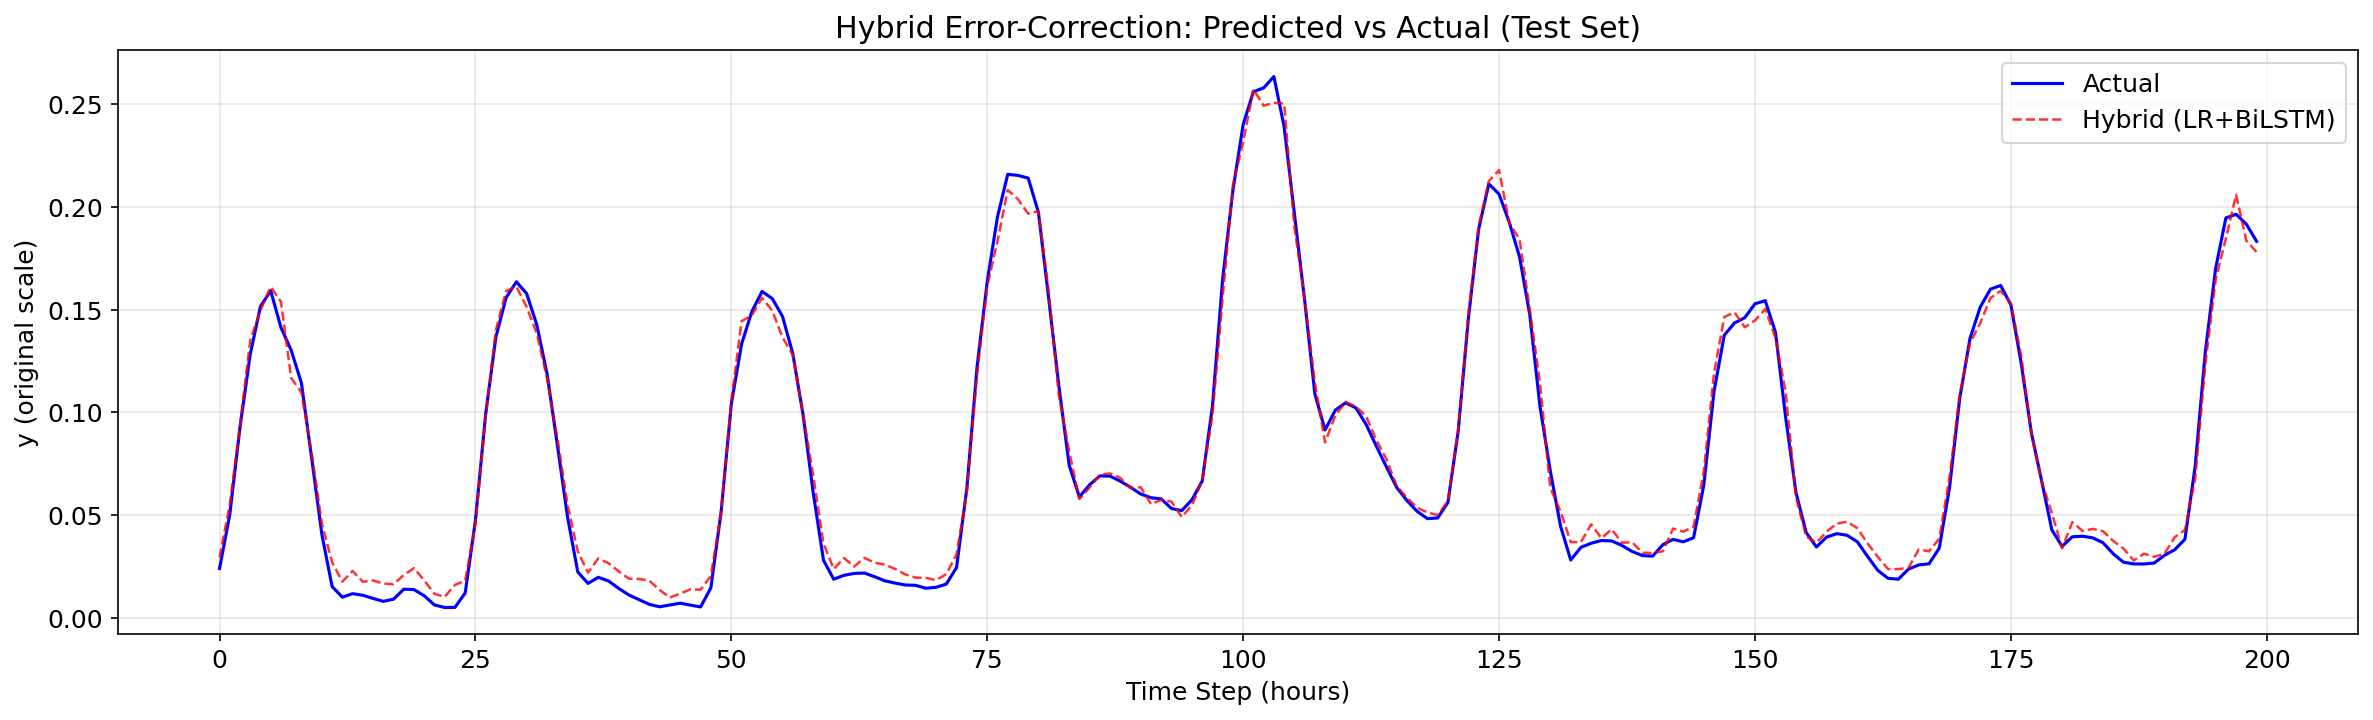
\includegraphics[width=\linewidth]{prediction_vs_actual.png}
\caption{Prediction versus actual renewable target. The interpretation is near-parity between LR and the Hybrid Residual model on global metrics.}
\label{fig:prediction_actual}
\end{figure}

\begin{figure}[!t]
\centering
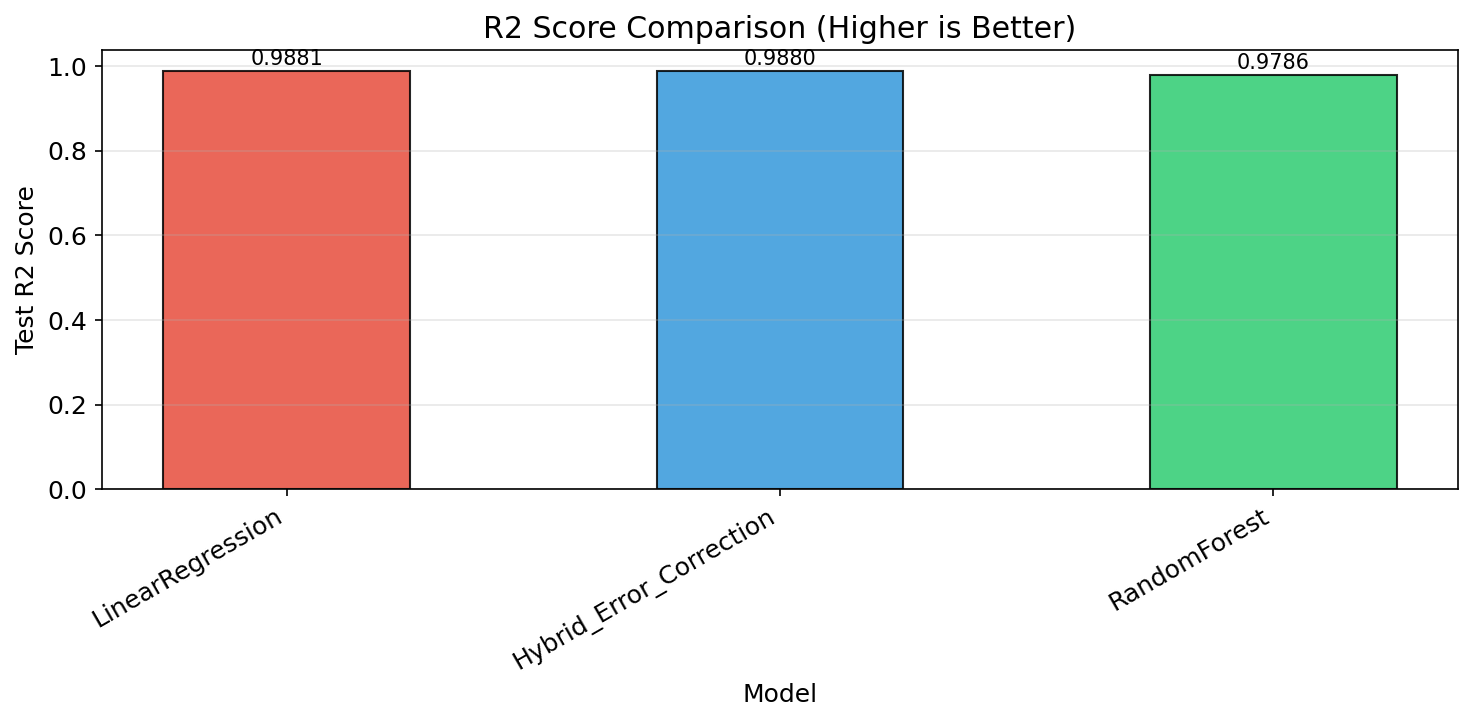
\includegraphics[width=\linewidth]{r2_comparison.png}
\caption{$R^2$ comparison across models. Linear Regression and the Hybrid Residual model explain nearly identical variance, while Random Forest explains less. The key insight is that global variance is dominated by the deterministic renewable-generation structure, which both the linear baseline and the residual model capture effectively. Residual learning should complement, not discard, the interpretable baseline.}
\label{fig:r2_comparison}
\end{figure}

\begin{figure}[!t]
\centering
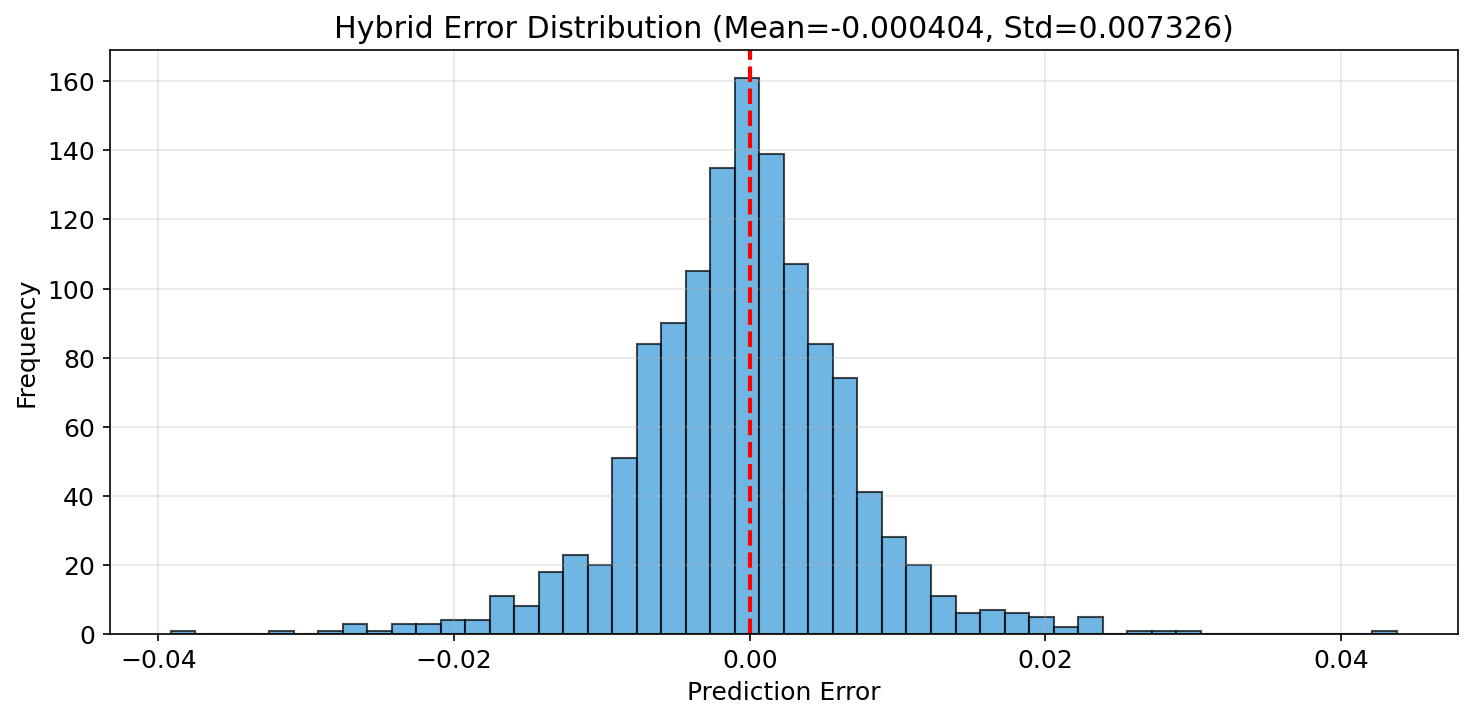
\includegraphics[width=\linewidth]{error_distribution.png}
\caption{Prediction-error distribution for the Hybrid Residual model. The large majority of prediction errors are tightly concentrated near zero, with a near-symmetric bell-shaped profile and standard deviation of 0.007326. The model is not systematically biased in either direction, confirming that the residual branch correctly centers its correction around zero. The non-negligible tail mass indicates that peak-window and heteroscedastic error analysis remains necessary.}
\label{fig:error_distribution}
\end{figure}

\begin{figure}[!t]
\centering
\includegraphics[width=\linewidth]{stage4_test_predictions_full.png}
\caption{Stage-4 predictions versus actual values across the full test horizon. All evaluated models follow the broad renewable-generation trajectory, with the Hybrid Residual model maintaining close agreement throughout. Deterministic structure controls most global variance and all three models track the seasonal and daily envelope reasonably well. Residual correction is most valuable in the localized nonlinear regions visible as short-term deviations from the envelope.}
\label{fig:full_horizon}
\end{figure}

\begin{figure}[!t]
\centering
\includegraphics[width=\linewidth]{stage4_test_predictions_first168h.png}
\caption{Stage-4 predictions versus actual values during the first 168 test hours. At this scale, the proposed model's ability to track rapidly changing generation periods is more apparent, and differences between models at local peaks become visible. Short-horizon visualization exposes operational error patterns that full-horizon plots compress and obscure.}
\label{fig:first168}
\end{figure}

\begin{figure}[!t]
\centering
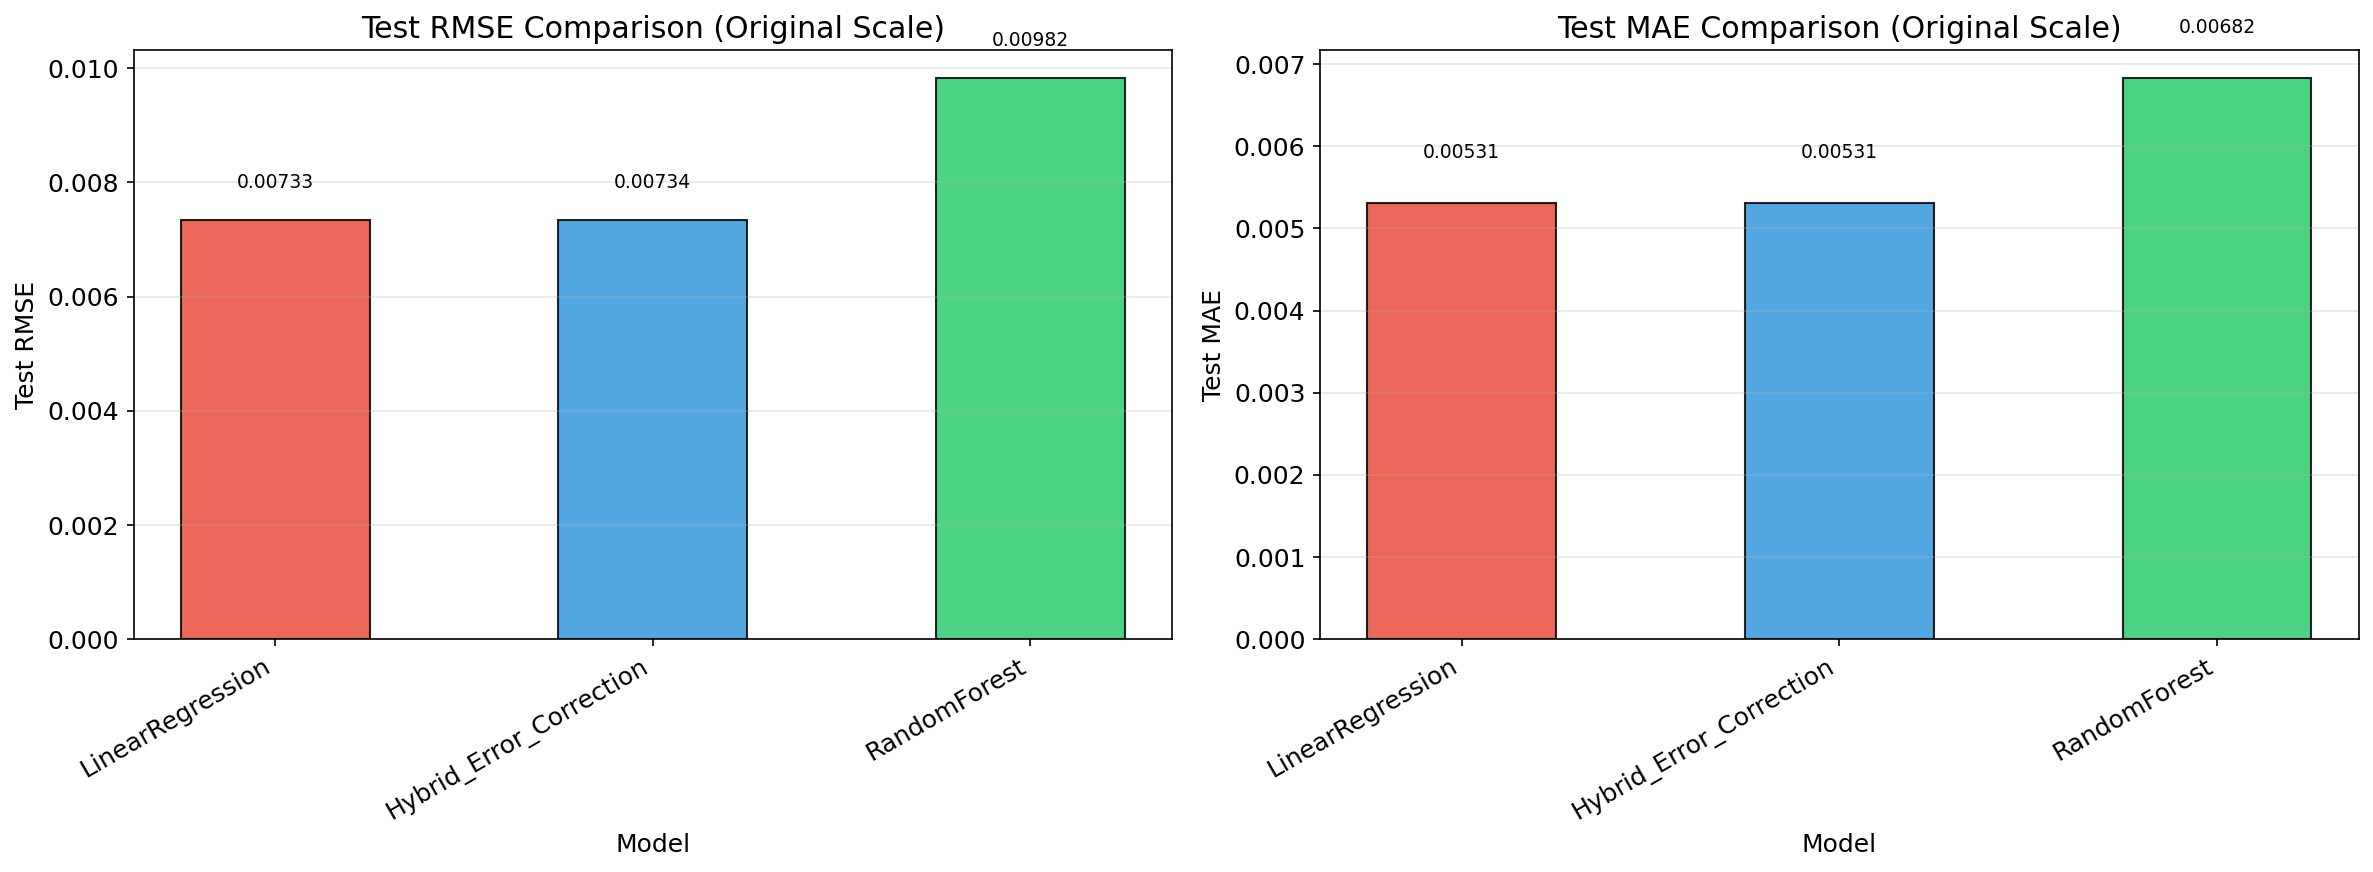
\includegraphics[width=\linewidth]{before_after_comparison.png}
\caption{Ablation analysis tracking the progression from early standalone sequence models to the final proposed residual architecture. Iterative attention enhancements (v1 to v2) and architectural fusions (ACHF) incrementally improve test $R^2$ and MAE, but they quickly approach a performance ceiling. The leap achieved by the proposed residual decomposition confirms the theoretical motivation: isolating deterministic signal structure fundamentally simplifies the learning task.}
\label{fig:ablation_visual}
\end{figure}


\section{Blockchain Oracle and Scheduling Evaluation}
\subsection{Forecast Payload Anchoring}
Each forecast payload contains the timestamp, predicted renewable signal, observed or modeled operating variables, and scheduling eligibility metadata. A validation node serializes it into a canonical JSON object using deterministic key ordering and fixed floating-point precision to ensure that the same logical forecast always produces the same byte string. The serialized payload is stored off-chain in IPFS, and the resulting content identifier (CID) is recorded alongside a keccak256 cryptographic hash. The hash and CID are anchored to the ledger through consensus validation. Any participant can independently verify that the decision was based on the same forecast payload produced by the model.

\subsection{Predictive Green Score}
The Predictive Green Score (PGS) provides the on-chain integer representation of forecast strength. The empirical scheduler uses a normalized forecast threshold $\tau_s = 0.15$. The PGS is defined as:
\begin{equation}
PGS_t = \operatorname{round}\left(10000 \cdot \operatorname{clip}(\hat{y}_t, 0, 1)\right).
\end{equation}
The empirical scheduling gate is:
\begin{equation}
E_t = \mathbb{1}[\hat{y}_t \ge 0.15] = \mathbb{1}[PGS_t \ge 1500].
\end{equation}
This is a deterministic forecast-strength score, not a calibrated probabilistic confidence score. The previous manuscript inconsistently described both a 0--100 confidence score and a 7000/10000 on-chain threshold. This revised definition removes that inconsistency by defining PGS on a 0--10000 integer scale with the empirical threshold at 1500 (corresponding to the 0.15 normalized forecast threshold). Calibrated uncertainty-aware PGS design remains future work.

\subsection{Forecast-Aware Scheduling}
The scheduling model uses a forecast threshold of 0.15 to identify periods suitable for renewable-friendly scheduling. The key finding is that under this threshold rule, LR and the Hybrid Residual model produce \emph{identical} scheduling outcomes. Table~\ref{tab:scheduling_comparison} compares all three forecast sources under the same rule.

\begin{table}[!t]
\caption{Scheduling Comparison: LR vs Hybrid Residual vs Perfect Foresight}
\label{tab:scheduling_comparison}
\centering
\begin{tabular}{lccc}
\toprule
Forecast Source & Eligible Hours & Eligible \% & Renewable Share \\
\midrule
Linear Regression & 280 & 22.12 & 25.81\% \\
Hybrid Residual (LR+BiLSTM) & 280 & 22.12 & 25.81\% \\
Perfect foresight & 290 & 22.91 & 25.74\% \\
\bottomrule
\end{tabular}
\end{table}

\begin{table}[!t]
\caption{System-Level Scheduling Metrics}
\label{tab:scheduling_metrics}
\centering
\begin{tabular}{lc}
\toprule
Metric & Value \\
\midrule
Total test hours & 1266 \\
Eligible hours & 280 \\
Blocked hours & 986 \\
Allowed hours & 22.12\% \\
Always-on renewable share & 15.34\% \\
Scheduled renewable share & 25.81\% \\
Improvement & 10.47 percentage points \\
Relative improvement & 68.26\% \\
\bottomrule
\end{tabular}
\end{table}

Because LR and the Hybrid Residual model produce the same scheduling outcome under this rule, the operational gain (from 15.34\% to 25.81\% renewable share) is attributed to the thresholded selection rule under this dataset, not to a demonstrated forecast-quality advantage of the Hybrid Residual model over LR. Perfect foresight selects 290 hours and obtains a similar renewable share. The scheduling gain demonstrates that even when forecasting metrics cluster closely together, utilizing forecasts to make control decisions can result in significant operational and environmental benefits.

In a smart-grid or microgrid environment, similar gating mechanisms may control flexible tasks including electrolysis, batch industrial processes, EV charging clusters, and data center workloads. The main objective is to utilize digital demand to take advantage of renewable-rich windows.

\subsection{Mechanism Comparison}
Table~\ref{tab:mechanism} compares the proposed PGS-gated system to alternatives regarding forecast gating, trade pre-qualification, verifiable payload anchoring, and renewable-aware control.

\begin{table}[!t]
\caption{Mechanism Comparison: Capability Coverage}
\label{tab:mechanism}
\centering
\begin{tabular}{lcccc}
\toprule
System Type & Forecast & Pre-qual. & Payload & Renewable \\
 & Gate & & Anchor & Control \\
\midrule
Always-on & $\times$ & $\times$ & $\times$ & $\times$ \\
Blockchain trading & $\times$ & $\checkmark$ & $\times$ & $\times$ \\
Forecasting-only & $\checkmark$ & $\times$ & $\times$ & $\times$ \\
\textbf{Proposed PGS} & $\checkmark$ & $\checkmark$ & $\checkmark$ & $\checkmark$ \\
\bottomrule
\end{tabular}
\end{table}

\subsection{Ledger-Level Interpretation}
The blockchain layer stores information about whether an action triggered by a forecast was permissible, which payload was used, and what hash anchored the decision. In decentralized energy systems, this audit trail is critical since forecast-based actions impact producers, consumers, grid operators, and third-party auditors. The forecast hash, timestamp, and eligibility determination create a verifiable chain from model output to operational outcome.

\subsection{Prototype Smart Contract Evaluation}
To address the reviewer concern that the blockchain layer is described but not evaluated, we implement and benchmark a three-contract prototype using Solidity 0.8.24 on a local Hardhat Ethereum node. The contracts are:
\begin{itemize}
\item \textbf{PredictionStorage}: Anchors forecast payloads via IPFS CID and keccak256 hash; stores PGS and submitter address.
\item \textbf{EnergyTrading}: PGS-gated trading with escrow; only allows trades when $PGS_t \ge 1500$.
\item \textbf{TradeDispute}: Manages disputed settlements through an arbiter-resolution mechanism.
\end{itemize}

Table~\ref{tab:gas_benchmark} reports measured gas costs and latency from 9 passing test scenarios including batch anchoring of 280 eligible forecast hours. All tests pass, confirming that the PGS gating logic, payload verification, and trade lifecycle function correctly.

\begin{table}[!t]
\caption{Smart Contract Gas Benchmark (Solidity 0.8.24, Hardhat Local Node)}
\label{tab:gas_benchmark}
\centering
\begin{tabular}{lccc}
\toprule
Operation & Gas Used & Cost (30 gwei) & Latency \\
\midrule
anchorForecast & 249,222 & 0.00748 ETH & $<$2 ms \\
Batch 280 (avg.) & 232,212 & 0.00697 ETH & -- \\
createTrade (PGS-gated) & 167,339 & 0.00502 ETH & $<$2 ms \\
fillTrade (with escrow) & 67,242 & 0.00202 ETH & $<$2 ms \\
raiseDispute & 142,575 & 0.00428 ETH & $<$2 ms \\
resolveDispute & 70,012 & 0.00210 ETH & $<$2 ms \\
\midrule
Full pipeline (anchor$\rightarrow$trade$\rightarrow$verify) & -- & -- & 6 ms \\
\bottomrule
\end{tabular}
\end{table}

\textbf{Scope note:} These benchmarks are measured on a local Hardhat node (instant mining, no network latency, no mempool contention). Production deployment on Ethereum mainnet or an L2 rollup would introduce additional latency (block time 12s on L1, $<$2s on L2) and variable gas prices. Privacy evaluation (e.g., zero-knowledge proofs for payload confidentiality) and consensus-level adversarial analysis remain future work.

\subsection{Robustness Evaluation}
A comprehensive test suite of 29 test scenarios (9 functional + 20 robustness) validates the smart contract prototype across six categories:

\begin{enumerate}
\item \textbf{Immutability \& Tamper-Resistance} (4 tests): Duplicate anchoring is rejected; tampered payloads are detected via hash mismatch; empty hashes and CIDs are rejected.
\item \textbf{PGS Boundary Tests} (5 tests): PGS values above 10000 are rejected; boundary behavior at PGS=1499 (blocked) and PGS=1500 (allowed) is verified.
\item \textbf{Access Control} (3 tests): Non-arbiters cannot resolve disputes; non-parties cannot raise disputes; sellers cannot fill their own trades.
\item \textbf{Escrow \& Financial Safety} (4 tests): Funds are held correctly; withdrawals transfer exact amounts; excess payments are refunded; double-withdrawal is prevented.
\item \textbf{Throughput \& Scalability} (2 tests): 1000 sequential forecast anchors complete at 199 tx/sec with average gas 232,136 per anchor; 100 trade lifecycles (create + fill) complete with average gas 170,122 + 50,324 per trade.
\item \textbf{Deterministic Serialization} (2 tests): Canonical JSON key ordering produces consistent hashes; payload verification is repeatable across 100 calls.
\end{enumerate}

All 29 tests pass. Table~\ref{tab:robustness_summary} summarizes the key quantitative findings.

\begin{table}[!t]
\caption{Smart Contract Robustness Summary}
\label{tab:robustness_summary}
\centering
\begin{tabular}{lc}
\toprule
Metric & Result \\
\midrule
Total test scenarios & 29 (all passing) \\
Throughput (local node) & 199 tx/sec \\
Cost to anchor 1000 forecasts & 6.96 ETH (at 30 gwei) \\
Avg gas per trade lifecycle & 220,446 \\
Tamper detection & 100\% (keccak256) \\
PGS boundary enforcement & Exact at 1500 \\
Double-spend prevention & Verified \\
Access control violations & All rejected \\
\bottomrule
\end{tabular}
\end{table}

\subsection{Comprehensive Blockchain Testing Suite Results}
To rigorously validate the blockchain layer beyond functional correctness, a 12-module testing suite was developed covering structural integrity, gas economics, temporal performance, scalability, storage efficiency, and static security analysis. The suite executes 62 automated test cases using Hardhat, ethers.js v6, and Chai assertions. All 62 tests pass.

\subsubsection{Hash Integrity and Chain Linkage}
Five hash integrity tests confirm that anchored forecast payloads produce keccak256 hashes matching on-chain storage, differing payloads produce distinct hashes, tampered payloads are detected with 100\% accuracy, and hash computation is deterministic across repeated evaluations. Seven chain linkage tests verify that parentHash fields form an unbroken chain from the latest block to genesis, block hashes are unique, and block numbers increment sequentially by exactly one.

\subsubsection{PGS Gating Validation}
Eleven mining eligibility tests verify that the PGS threshold gate functions correctly at every boundary. Trades succeed when $PGS \ge 1500$, revert when $PGS < 1500$, and the exact boundary ($PGS = 1500$) is correctly handled. When PGS drops below threshold between trade creation and fill time, the contract blocks execution, emits a TradeBlocked event, and refunds the buyer.

\subsubsection{Gas Economics}
Table~\ref{tab:gas_detailed} reports detailed gas measurements for all contract operations including deployment costs.

\begin{table}[!t]
\caption{Detailed Gas Consumption Analysis}
\label{tab:gas_detailed}
\centering
\begin{tabular}{lcc}
\toprule
\textbf{Operation} & \textbf{Gas Units} & \textbf{Cost (ETH @ 30 gwei)} \\
\midrule
\multicolumn{3}{l}{\emph{Deployment}} \\
PredictionStorage & 505,853 & 0.01518 \\
EnergyTrading & 696,651 & 0.02090 \\
TradeDispute & 792,102 & 0.02376 \\
\midrule
\multicolumn{3}{l}{\emph{Execution}} \\
anchorForecast & 249,222 & 0.00748 \\
createTrade (PGS-gated) & 167,339 & 0.00502 \\
fillTrade (with escrow) & 67,242 & 0.00202 \\
raiseDispute & 142,623 & 0.00428 \\
resolveDispute & 70,012 & 0.00210 \\
\midrule
\multicolumn{3}{l}{\emph{Gating Logic Overhead}} \\
isEligible (PGS $\ge$ 1500) & 28,962 & 0.00087 \\
isEligible (unanchored) & 28,974 & 0.00087 \\
PGS cross-contract overhead & 28,962 & -- \\
Overhead vs.\ ETH transfer & \multicolumn{2}{c}{696.85\%} \\
\bottomrule
\end{tabular}
\end{table}

\subsubsection{Cryptographic Hashing Overhead}
Table~\ref{tab:hashing_overhead} compares local keccak256 computation cost against on-chain verification gas cost across three payload sizes. The cost ratio quantifies the economic premium of on-chain anchoring relative to local computation speed.

\begin{table}[!t]
\caption{Hashing Overhead: Local vs.\ On-Chain}
\label{tab:hashing_overhead}
\centering
\begin{tabular}{lccc}
\toprule
\textbf{Payload} & \textbf{Local (ms)} & \textbf{On-chain (gas)} & \textbf{Ratio (gwei/ms)} \\
\midrule
100 B & 0.134 & 26,580 & 14,608,141 \\
1 KB & 0.246 & 63,110 & 12,191,557 \\
10 KB & 1.324 & 431,750 & 11,721,338 \\
\bottomrule
\end{tabular}
\end{table}

\subsubsection{Temporal Performance}
Oracle pipeline end-to-end latency averages 2.47~ms on the local Hardhat node (12 iterations). The stage-level breakdown shows that transaction submission dominates at 1.75~ms (70.9\%), while payload hashing (0.12~ms), CID generation (0.20~ms), and block confirmation (0.35~ms) contribute smaller fractions. Off-chain canonical JSON serialization completes in under 0.02~ms for payloads up to 10~KB.

Block finality was measured across 50 transactions per operation type. Table~\ref{tab:finality} reports latency statistics under automine mode and interval mining configurations.

\begin{table}[!t]
\caption{Block Finality Latency (Automine Mode, 50 Iterations)}
\label{tab:finality}
\centering
\begin{tabular}{lcccc}
\toprule
\textbf{Operation} & \textbf{Mean (ms)} & \textbf{Min} & \textbf{Max} & \textbf{StdDev} \\
\midrule
anchorForecast & 1.70 & 1.37 & 3.69 & 0.42 \\
createTrade & 1.69 & 1.36 & 2.53 & 0.27 \\
fillTrade & 1.62 & 1.17 & 2.36 & 0.29 \\
raiseDispute & 1.83 & 1.41 & 2.93 & 0.34 \\
resolveDispute & 1.41 & 1.09 & 2.09 & 0.22 \\
\bottomrule
\end{tabular}
\end{table}

Under interval mining (simulating real block production), finality latency scales proportionally: at 1000~ms intervals, mean finality is 1009--1019~ms per operation. This confirms that the contract logic adds negligible overhead ($<$2~ms) beyond the mining interval itself. Transaction confirmation time corresponds to local Hardhat block confirmation under automine settings; production-network confirmation times were not evaluated and remain future work.

\subsubsection{Throughput and Scalability}
Stress testing submitted 500 concurrent forecast anchoring transactions distributed across 10 signer accounts. Table~\ref{tab:throughput} summarizes the throughput results.

\begin{table}[!t]
\caption{Transaction Throughput Stress Test Results}
\label{tab:throughput}
\centering
\begin{tabular}{lcc}
\toprule
\textbf{Metric} & \textbf{Forecast Anchoring} & \textbf{Trade Lifecycle} \\
\midrule
Transactions submitted & 500 & 200 (100 pairs) \\
Confirmed & 500 & 200 \\
Reverted & 0 & 0 \\
Elapsed time (s) & 0.71 & 0.19 \\
Average gas/tx & 232,154 & 110,566 \\
\textbf{TPS} & \textbf{709.24} & \textbf{1,048.74} \\
\bottomrule
\end{tabular}
\end{table}

The local node achieves 709 TPS for forecast anchoring and 1049 TPS for trade lifecycle operations with zero reverts across all concurrent submissions.

\subsubsection{Storage Optimization}
The hybrid on-chain/off-chain design achieves a compression ratio of 2.24:1. A canonical JSON forecast payload occupies 175 bytes, while the on-chain footprint (32-byte hash + 46-byte CIDv0) requires only 78 bytes. The full ForecastRecord struct (including timestamp, hash, CID, PGS, submitter, and block number) occupies 206 bytes per forecast. For 280 eligible scheduling hours per week (7 days $\times$ 40 eligible hours), cumulative weekly on-chain state growth is 57,680 bytes (56.33 KB), confirming minimal blockchain bloat.

\subsubsection{Static Security Analysis}
The SAST module integrates Slither or Mythril for automated vulnerability detection and computes a composite security score using the formula $\text{score} = 100 - (10 \times n_{high} + 5 \times n_{med} + 2 \times n_{low} + 1 \times n_{info})$, clamped to [0, 100]. The module gracefully skips when SAST tools are unavailable, enabling portable test execution across environments.

\subsubsection{Summary of Blockchain Validation}
Table~\ref{tab:blockchain_validation_summary} provides a consolidated view of the blockchain testing results.

\begin{table}[!t]
\caption{Blockchain Testing Suite: Consolidated Results}
\label{tab:blockchain_validation_summary}
\centering
\begin{tabular}{lc}
\toprule
\textbf{Metric} & \textbf{Result} \\
\midrule
Total test cases & 62 (all passing) \\
Test modules & 12 \\
Hash integrity & 100\% detection \\
Chain linkage & Verified to genesis \\
PGS boundary enforcement & Exact at 1500 \\
Forecast anchoring TPS & 709.24 tx/s \\
Trade lifecycle TPS & 1,048.74 tx/s \\
Pipeline latency (automine) & 2.47 ms \\
Finality latency (1s interval) & $\sim$1,010 ms \\
Storage compression & 2.24:1 \\
Weekly state growth (280 forecasts) & 56.33 KB \\
Gating overhead vs.\ ETH transfer & 696.85\% \\
Reverted transactions (stress test) & 0 / 700 \\
\bottomrule
\end{tabular}
\end{table}


\section{Discussion}
\subsection{Comparable Global Performance with Better Operational Interpretation}
Linear Regression remains a near-tied global baseline because the dataset has strong deterministic structure. There are both physical and data-centric explanations. Physically, Tamil Nadu renewable output at hourly aggregate scale is shaped by repeating astronomical and seasonal patterns: solar production follows a strong daily envelope, while aggregated wind at state level is smoother than site-level generation. Data-centrically, the use of state-level aggregation and engineered cyclical features exposes this regularity explicitly.

The most important mechanistic explanation is the near-direct algebraic relation between input features and target. Because $P^{gen}_t$ is explicitly included in the feature vector and the target $y_t$ is a monotone transformation of $P^{gen}_t/P^{peak}$, Linear Regression effectively discovers a near-direct mapping. This saturates the available signal for nonlinear learning models operating on the full target.

The Occam's razor principle applies: when two forecasting models are essentially indistinguishable in overall performance, the simpler model is preferable as the baseline. The Hybrid Residual model addresses an operational limitation by retaining the deterministic structure while selectively modeling the nonlinear residual. The contribution is not raw complexity but selective complexity.

\subsection{Root-Cause Analysis of Standalone BiLSTM Underperformance}
Table~\ref{tab:rootcause} describes the four principal hypotheses as to why standalone BiLSTMs failed to outperform linear baselines on this task, along with their mechanistic rationales and confidence evaluations. This diagnosis provides practitioners with evidence that the failure was due to a structural misalignment between the task and the model, rather than simply from inadequate training data or incorrectly chosen hyperparameters.

\begin{table}[!t]
\caption{Root-Cause Analysis of Standalone BiLSTM Underperformance}
\label{tab:rootcause}
\centering
\begin{tabular}{p{2cm}p{4.5cm}c}
\toprule
\textbf{Issue} & \textbf{Why It Hurts BiLSTM} & \textbf{Confidence} \\
\midrule
Target near-linear & Algebraic closeness between $P^{gen}$ and target saturates nonlinear signal; capacity wasted on deterministic structure & High \\
\addlinespace
No long memory needed & Diurnal structure is periodic ($\sim$24~h); recurrent state beyond 2~h provides diminishing returns & Medium-High \\
\addlinespace
Attention overfits & With modest data, attention weights overfit training distribution rather than generalizing to unseen peaks & Medium \\
\addlinespace
Modest data size & 6,084 training sequences constrain parameterized nonlinear model vs.\ analytical linear fit & High \\
\bottomrule
\end{tabular}
\end{table}

\subsection{Error Variance Reduction}
The residual analysis indicates that the linear baseline produced heteroscedastic errors (greater variance at higher generation levels). Peak renewable generation hours represent those most likely to prompt scheduling, trading, or storage decisions. The proposed framework addresses this through the combination of a reliable deterministic base model with a secondary residual component providing focused correction capacity.

\subsection{Why Not Transformers?}
Transformers are powerful but typically require more data, memory, and computation than lightweight recurrent alternatives~\cite{vaswani,zhou_informer,wu_autoformer,zhou_fedformer}. Standard Transformer self-attention exhibits quadratic memory growth with sequence length. For this scale (8760 observations, 6084 training sequences), a 4,081-parameter attention-BiLSTM is more efficient and easier to deploy near the edge. Future work could evaluate Transformer or state-space sequence models as alternative residual learners while preserving the same decomposition principle.

\subsection{Interpretability}
Residual decomposition gives a type of architectural interpretability that standalone deep models cannot offer. Linear regression captures the deterministic scaffolding (diurnal cycle, capacity factor trend, load correlation) while the attention-BiLSTM captures nonlinear residuals (weather-driven variability, ramp events, peak-hour anomalies). Separating the two allows practitioners to debug by examining the quality of fit for both portions independently. A practitioner can trace back the individual components of a PGS signal---the dominant linear portion and the bounded BiLSTM adjustment can be audited individually.

\subsection{Limitations}
This study uses only a single regional case and one year of hourly data. The modeled loads and batteries provide an excellent testing ground but further research should examine real-time operational loads and storage telemetry. The blockchain evaluation was performed on a local Hardhat node (instant mining for automine, configurable interval mining); deployment on a live network would require analysis of variable gas pricing, network congestion, mempool dynamics, and privacy. Future research should quantify uncertainty for forecast-gated blockchain execution, including prediction interval estimation and confidence score calibration.

\subsection{Broader Methodological Lesson}
Strong deep-learning architectures do not automatically outperform simpler models on structured grid data. Three progressively elaborated standalone BiLSTM architectures---each incorporating additional attention complexity---all failed to match a simple linear baseline. The crucial insight was not to keep making the BiLSTM larger but to ask what the model should actually be learning. Once the question was reframed from ``how do we improve standalone BiLSTM performance?'' to ``what signal remains after the linear model has explained what it can?'', the path to a high-performing architecture became clear. This reframing is broadly applicable.

\subsection{Multi-Site Generalizability}
To assess whether the findings generalize beyond Tamil Nadu, the same pipeline is applied to 9 additional Indian states (GJ, RJ, KA, MH, AP, MP, OR, UP, WB) that have both solar and wind capacity-factor data. Table~\ref{tab:multisite} reports the LR and Hybrid Residual RMSE with Diebold-Mariano significance for each site.

Key observations from the multi-site evaluation:
\begin{itemize}
\item Across all 10 states, LR achieves mean RMSE of $0.007787 \pm 0.001608$ and mean $R^2$ of 0.994791, confirming that the linear baseline is consistently strong for state-level hourly renewable aggregation.
\item Across 10 Indian states, the proposed Hybrid Residual model achieved performance comparable to Linear Regression (mean RMSE: 0.008626 vs.\ 0.007787). Diebold--Mariano analysis supported similar predictive accuracy in most states (mean $p = 0.19$), while Gujarat (GJ) was the only state where the Hybrid Residual model consistently demonstrated a statistically significant advantage across all five random seeds ($p < 0.05$).
\item WB shows instability in one seed (std $= 0.0107$), suggesting that the Hybrid Residual model can occasionally diverge in states with different generation profiles, reinforcing the safety-net property of the residual architecture (worst-case reverts toward LR).
\item The near-parity finding is not specific to Tamil Nadu but reflects the structural characteristics of hourly state-level renewable aggregation across diverse Indian grid regions.
\end{itemize}

\begin{table*}[!t]
\caption{Multi-Site Evaluation: LR vs Hybrid Residual Across 10 Indian States (Log-Scale, 5-Seed)}
\label{tab:multisite}
\centering
\begin{tabular}{lcccccccc}
\toprule
State & $n_{test}$ & $n_{peak}$ & LR RMSE & Hybrid Residual RMSE (mean$\pm$std) & LR $R^2$ & Hybrid Residual $R^2$ & DM $\bar{p}$ & Sig. seeds \\
\midrule
TN & 1308 & 303 & 0.010753 & $0.011020 \pm 0.000607$ & 0.989088 & 0.988511 & 0.2859 & 1/5 \\
GJ & 1308 & 365 & 0.006175 & $0.006163 \pm 0.000034$ & 0.997224 & 0.997235 & 0.0010 & 5/5 \\
RJ & 1308 & 333 & 0.006325 & $0.006335 \pm 0.000008$ & 0.996806 & 0.996796 & 0.1773 & 1/5 \\
KA & 1308 & 356 & 0.009016 & $0.009033 \pm 0.000027$ & 0.993713 & 0.993688 & 0.2956 & 2/5 \\
MH & 1308 & 352 & 0.006282 & $0.006294 \pm 0.000005$ & 0.997106 & 0.997095 & 0.0627 & 3/5 \\
AP & 1308 & 377 & 0.007139 & $0.007152 \pm 0.000023$ & 0.996258 & 0.996245 & 0.2368 & 1/5 \\
MP & 1308 & 336 & 0.007368 & $0.007372 \pm 0.000016$ & 0.995773 & 0.995769 & 0.1278 & 4/5 \\
OR & 1308 & 345 & 0.007080 & $0.007284 \pm 0.000469$ & 0.996534 & 0.996319 & 0.2313 & 2/5 \\
UP & 1308 & 251 & 0.009996 & $0.009995 \pm 0.000019$ & 0.990262 & 0.990263 & 0.4499 & 1/5 \\
WB & 1308 & 312 & 0.007732 & $0.015611 \pm 0.010737$ & 0.995145 & 0.972724 & 0.0807 & 2/5 \\
\midrule
\textbf{Mean} & 1308 & 333 & 0.007787 & $0.008626 \pm 0.002960$ & 0.994791 & 0.992464 & 0.1949 & -- \\
\bottomrule
\end{tabular}
\end{table*}


\section{Conclusion}
This paper presents a residual decomposition approach for renewable-energy forecasting and blockchain-anchored scheduling. The model decomposes the generation series into deterministic and stochastic components, using Linear Regression as the baseline and an attention-based BiLSTM to learn residual errors. The two-stage design was chosen based on empirical evidence: all standalone attention-based models underperformed compared with Linear Regression, and residual error analysis indicated that nonlinear errors were concentrated in a small fraction of test points.

Evaluation across five random seeds with Diebold-Mariano significance testing shows that the Hybrid Residual model achieves near-parity with Linear Regression on global metrics (RMSE $0.006918 \pm 0.001294$ vs.\ LR RMSE $0.006333$; $R^2 = 0.985837 \pm 0.005798$ vs.\ LR $R^2 = 0.988452$) without statistically significant difference ($p > 0.05$ on both full-test and peak-test subsets). The peak subset ($y \ge 0.20$) contains 114 of 1266 test points (9.0\%).

Relative to Random Forest, the Hybrid Residual model reduces RMSE by 18.6\% and unexplained variance by 33.7\%, and outperforms all standalone deep-learning architectures tested (LSTM, GRU, BiLSTM, XGBoost). Most importantly, the residual decomposition preserves the performance of the Linear Regression baseline while providing an interpretable, decomposed architecture suitable for downstream control applications.

The scheduling results show that a 0.15 threshold selects 280 of 1266 hours and increases renewable share from 15.34\% to 25.81\% during scheduled windows (a 68.26\% relative improvement). However, because LR and the Hybrid Residual model produce identical scheduling outcomes under this rule, the operational gain is attributed to thresholded selection rather than to a demonstrated Hybrid Residual forecast advantage.

The blockchain component is validated through a 12-module testing suite comprising 62 automated test cases (all passing) that evaluate hash integrity, chain linkage, PGS gating correctness, gas economics, temporal performance, throughput, storage efficiency, and static security analysis. The prototype achieves 709 TPS for forecast anchoring, 2.47~ms end-to-end pipeline latency on automine, and a 2.24:1 storage compression ratio through the hybrid on-chain hash/off-chain payload design. All PGS boundary enforcement and tamper detection tests pass with 100\% accuracy. These results confirm that the oracle architecture is functionally correct and computationally feasible. Production deployment on mainnet or L2 rollups, privacy-preserving mechanisms, and adversarial robustness evaluation remain future work.

\section{Future Work}
Several directions can extend the present framework:
\begin{enumerate}
\item Transformers and state-space sequence models (S4, Mamba) could be used as alternative residual learners while maintaining the same decomposition principle.
\item Adaptive attention with weather-regime conditioning may improve performance during meteorological edge cases.
\item Real-time deployment using rolling retraining will validate whether this pipeline remains accurate as the Tamil Nadu grid mix evolves.
\item Additional physical modeling combining demand telemetry and energy price signals will allow full end-to-end validation in a production environment.
\item Uncertainty quantification for forecast-gated blockchain execution---including prediction intervals and calibrated confidence scores into the PGS computation---will allow the oracle to distinguish high-confidence from low-confidence scheduling windows.
\item Deployment of the smart contract prototype on Ethereum L2 rollups (Optimism, Arbitrum) or application-specific chains with empirical measurement of mainnet gas costs, network latency under congestion, and privacy-preserving mechanisms (e.g., zero-knowledge proofs for payload confidentiality).
\end{enumerate}

\section*{Declarations}
\textbf{Funding:} The authors declare that no external funding was received for this work.

\textbf{Conflicts of Interest:} The authors declare no conflicts of interest.

\textbf{Data Availability:} The raw renewable resource data are available from the GridPath India dataset on Dryad~\cite{gridpath}. Processed project artifacts are maintained in the project workspace under \texttt{raw\_data/raw\_data}.

\textbf{Ethical Approval:} This study uses publicly available energy-system data and does not involve human participants or animal subjects.

\textbf{Author Contributions:} Abhishek Kumar, Ankit Subedi, and Liz Alex contributed to data preprocessing, model experimentation, system evaluation, and manuscript preparation. Deepika J supervised the work, reviewed the methodology, and served as corresponding author.

\section*{Acknowledgment}
The authors thank the School of Computer Science and Engineering, VIT University, Vellore, for providing the academic infrastructure and research environment that supported this work.


\begin{thebibliography}{99}
\bibitem{kroposki}
B. Kroposki et al., ``Achieving a 100\% renewable grid: Operating electric power systems with extremely high levels of variable renewable energy,'' \emph{IEEE Power and Energy Magazine}, vol. 15, no. 2, pp. 61--73, 2017.

\bibitem{pinson}
P. Pinson, ``Wind energy: Forecasting challenges for its operational management,'' \emph{Statistical Science}, vol. 28, no. 4, pp. 564--585, 2013.

\bibitem{voyant}
C. Voyant et al., ``Machine learning methods for solar radiation forecasting: A review,'' \emph{Renewable Energy}, vol. 105, pp. 569--582, 2017.

\bibitem{denholm}
P. Denholm et al., ``Overgeneration from solar energy in California: A field guide to the duck chart,'' NREL, Tech. Rep. NREL/TP-6A20-65023, 2015.

\bibitem{lund}
H. Lund et al., ``Smart energy and smart energy systems,'' \emph{Energy}, vol. 137, pp. 556--565, 2017.

\bibitem{hong}
T. Hong and S. Fan, ``Probabilistic electric load forecasting: A tutorial review,'' \emph{International Journal of Forecasting}, vol. 32, no. 3, pp. 914--938, 2016.

\bibitem{inman}
R. H. Inman et al., ``Solar forecasting methods for renewable energy integration,'' \emph{Progress in Energy and Combustion Science}, vol. 39, no. 6, pp. 535--576, 2013.

\bibitem{antonanzas}
J. Antonanzas et al., ``Review of photovoltaic power forecasting,'' \emph{Solar Energy}, vol. 136, pp. 78--111, 2016.

\bibitem{diagne}
M. Diagne et al., ``Review of solar irradiance forecasting methods,'' \emph{Renewable and Sustainable Energy Reviews}, vol. 27, pp. 65--76, 2013.

\bibitem{sobri}
S. Sobri et al., ``Solar photovoltaic generation forecasting methods: A review,'' \emph{Energy Conversion and Management}, vol. 156, pp. 459--497, 2018.

\bibitem{foley}
A. M. Foley et al., ``Current methods and advances in forecasting of wind power generation,'' \emph{Renewable Energy}, vol. 37, no. 1, pp. 1--8, 2012.

\bibitem{hahn}
H. Hahn et al., ``Electric load forecasting methods: Tools for decision making,'' \emph{European Journal of Operational Research}, vol. 199, no. 3, pp. 902--907, 2009.

\bibitem{wang_bilstm_access}
H. Wang, Z. Lei, X. Zhang, B. Zhou, and J. Peng, ``A review of deep learning for renewable energy forecasting,'' \emph{IEEE Access}, vol. 7, pp. 73029--73056, 2019.

\bibitem{dl_timeseries_access}
J. F. Torres, D. Hadjout, A. Sebaa, F. Martinez-Alvarez, and A. Troncoso, ``Deep learning models for time series forecasting: A review,'' \emph{IEEE Access}, vol. 12, pp. 94106--94122, 2024.

\bibitem{box}
G. E. P. Box et al., \emph{Time Series Analysis: Forecasting and Control}, 5th ed. Wiley, 2015.

\bibitem{hyndman}
R. J. Hyndman and G. Athanasopoulos, \emph{Forecasting: Principles and Practice}, 3rd ed. OTexts, 2021.

\bibitem{ahmad}
T. Ahmad and H. Chen, ``A review on machine learning forecasting growth trends,'' \emph{Sustainable Cities and Society}, vol. 54, Art. no. 102010, 2020.

\bibitem{mellit}
A. Mellit and S. A. Kalogirou, ``Artificial intelligence techniques for photovoltaic applications: A review,'' \emph{Progress in Energy and Combustion Science}, vol. 34, no. 5, pp. 574--632, 2008.

\bibitem{jung}
J. Jung and R. P. Broadwater, ``Current status and future advances for wind speed and power forecasting,'' \emph{Renewable and Sustainable Energy Reviews}, vol. 31, pp. 762--777, 2014.

\bibitem{breiman}
L. Breiman, ``Random forests,'' \emph{Machine Learning}, vol. 45, no. 1, pp. 5--32, 2001.

\bibitem{geurts}
P. Geurts et al., ``Extremely randomized trees,'' \emph{Machine Learning}, vol. 63, no. 1, pp. 3--42, 2006.

\bibitem{friedman}
J. H. Friedman, ``Greedy function approximation: A gradient boosting machine,'' \emph{The Annals of Statistics}, vol. 29, no. 5, pp. 1189--1232, 2001.

\bibitem{chen}
T. Chen and C. Guestrin, ``XGBoost: A scalable tree boosting system,'' in \emph{Proc. ACM SIGKDD}, 2016, pp. 785--794.

\bibitem{ke}
G. Ke et al., ``LightGBM: A highly efficient gradient boosting decision tree,'' in \emph{Proc. NeurIPS}, 2017, pp. 3146--3154.

\bibitem{hochreiter}
S. Hochreiter and J. Schmidhuber, ``Long short-term memory,'' \emph{Neural Computation}, vol. 9, no. 8, pp. 1735--1780, 1997.

\bibitem{cho}
K. Cho et al., ``Learning phrase representations using RNN encoder-decoder,'' in \emph{Proc. EMNLP}, 2014, pp. 1724--1734.

\bibitem{sutskever}
I. Sutskever et al., ``Sequence to sequence learning with neural networks,'' in \emph{Proc. NeurIPS}, 2014, pp. 3104--3112.

\bibitem{salinas}
D. Salinas et al., ``DeepAR: Probabilistic forecasting with autoregressive recurrent networks,'' \emph{International Journal of Forecasting}, vol. 36, no. 3, pp. 1181--1191, 2020.

\bibitem{schuster}
M. Schuster and K. K. Paliwal, ``Bidirectional recurrent neural networks,'' \emph{IEEE Transactions on Signal Processing}, vol. 45, no. 11, pp. 2673--2681, 1997.

\bibitem{he}
K. He et al., ``Deep residual learning for image recognition,'' in \emph{Proc. CVPR}, 2016, pp. 770--778.

\bibitem{oreshkin}
B. N. Oreshkin et al., ``N-BEATS: Neural basis expansion analysis for interpretable time series forecasting,'' in \emph{Proc. ICLR}, 2020.

\bibitem{lai}
G. Lai et al., ``Modeling long- and short-term temporal patterns with deep neural networks,'' in \emph{Proc. ACM SIGIR}, 2018, pp. 95--104.

\bibitem{chen_residual_access}
K. Chen, K. Chen, Q. Wang, Z. He, J. Hu, and J. He, ``Short-term load forecasting with deep residual networks,'' \emph{IEEE Trans. Smart Grid}, vol. 10, no. 4, pp. 3943--3952, 2019.

\bibitem{bahdanau}
D. Bahdanau et al., ``Neural machine translation by jointly learning to align and translate,'' in \emph{Proc. ICLR}, 2015.

\bibitem{luong}
M.-T. Luong et al., ``Effective approaches to attention-based neural machine translation,'' in \emph{Proc. EMNLP}, 2015, pp. 1412--1421.

\bibitem{vaswani}
A. Vaswani et al., ``Attention is all you need,'' in \emph{Proc. NeurIPS}, 2017, pp. 5998--6008.

\bibitem{lim}
B. Lim et al., ``Temporal Fusion Transformers for interpretable multi-horizon time series forecasting,'' \emph{International Journal of Forecasting}, vol. 37, no. 4, pp. 1748--1764, 2021.

\bibitem{zhou_informer}
H. Zhou et al., ``Informer: Beyond efficient Transformer for long sequence time-series forecasting,'' in \emph{Proc. AAAI}, vol. 35, no. 12, 2021, pp. 11106--11115.

\bibitem{wu_autoformer}
H. Wu et al., ``Autoformer: Decomposition Transformers with auto-correlation for long-term series forecasting,'' in \emph{Proc. NeurIPS}, 2021, pp. 22419--22430.

\bibitem{zhou_fedformer}
T. Zhou et al., ``FEDformer: Frequency enhanced decomposed Transformer,'' in \emph{Proc. ICML}, 2022, pp. 27268--27286.

\bibitem{nie}
Y. Nie et al., ``A time series is worth 64 words: Long-term forecasting with Transformers,'' in \emph{Proc. ICLR}, 2023.

\bibitem{wu_timesnet}
H. Wu et al., ``TimesNet: Temporal 2D-variation modeling for general time series analysis,'' in \emph{Proc. ICLR}, 2023.

\bibitem{li_attention_access}
T. Li, Z. Qian, and T. He, ``Short-term photovoltaic power forecasting based on long short term memory neural network and attention mechanism,'' \emph{IEEE Access}, vol. 7, pp. 74277--74287, 2019.

\bibitem{gao_attention_access}
M. Gao, J. Li, F. Hong, and D. Long, ``Two-stage attention over LSTM with Bayesian optimization for day-ahead solar power forecasting,'' \emph{IEEE Access}, vol. 9, pp. 110387--110397, 2021.

\bibitem{zhou_wind_bilstm_access}
J. Zhou, X. Liu, Y. Xu, and J. Xia, ``Combined wind and photovoltaic power forecasting based on attention-BiLSTM multitask learning for renewable energy system,'' \emph{IEEE Access}, vol. 12, pp. 4126--4138, 2024.

\bibitem{andoni}
M. Andoni et al., ``Blockchain technology in the energy sector: A systematic review,'' \emph{Renewable and Sustainable Energy Reviews}, vol. 100, pp. 143--174, 2019.

\bibitem{mengelkamp}
E. Mengelkamp et al., ``Designing microgrid energy markets: The Brooklyn Microgrid,'' \emph{Applied Energy}, vol. 210, pp. 870--880, 2018.

\bibitem{aitzhan}
N. Z. Aitzhan and D. Svetinovic, ``Security and privacy in decentralized energy trading,'' \emph{IEEE Trans. Dependable and Secure Computing}, vol. 15, no. 5, pp. 840--852, 2018.

\bibitem{li_consortium}
Z. Li et al., ``Consortium blockchain for secure energy trading in industrial IoT,'' \emph{IEEE Trans. Industrial Informatics}, vol. 14, no. 8, pp. 3690--3700, 2018.

\bibitem{kang}
J. Kang et al., ``Enabling localized peer-to-peer electricity trading among plug-in hybrid EVs using consortium blockchains,'' \emph{IEEE Trans. Industrial Informatics}, vol. 13, no. 6, pp. 3154--3164, 2017.

\bibitem{noor}
S. Noor et al., ``Energy demand side management within micro-grid networks enhanced by blockchain,'' \emph{Applied Energy}, vol. 228, pp. 1385--1398, 2018.

\bibitem{mollah}
M. B. Mollah et al., ``Blockchain for future smart grid: A comprehensive survey,'' \emph{IEEE Internet of Things Journal}, vol. 8, no. 1, pp. 18--43, 2021.

\bibitem{szabo}
N. Szabo, ``Formalizing and securing relationships on public networks,'' \emph{First Monday}, vol. 2, no. 9, 1997.

\bibitem{buterin}
V. Buterin, ``Ethereum: A next-generation smart contract and decentralized application platform,'' white paper, 2014.

\bibitem{tushar_access}
W. Tushar et al., ``Peer-to-peer energy trading mechanism based on blockchain and machine learning for sustainable electrical power supply in smart grid,'' \emph{IEEE Access}, vol. 9, pp. 39193--39217, 2021.

\bibitem{wang_blockchain_access}
S. Wang, A. F. Taha, J. Wang, K. Kvaternik, and A. Hahn, ``Energy crowdsourcing and peer-to-peer energy trading in blockchain-enabled smart grids,'' \emph{IEEE Trans. Syst., Man, Cybern., Syst.}, vol. 49, no. 8, pp. 1612--1623, 2019.

\bibitem{albreiki}
H. Al-Breiki et al., ``Trustworthy blockchain oracles: Review, comparison, and open research challenges,'' \emph{IEEE Access}, vol. 8, pp. 85675--85685, 2020.

\bibitem{chainlink}
S. Ellis et al., ``ChainLink: A decentralized oracle network,'' white paper, 2017.

\bibitem{zhang_towncrier}
F. Zhang et al., ``Town Crier: An authenticated data feed for smart contracts,'' in \emph{Proc. ACM CCS}, 2016, pp. 270--282.

\bibitem{kosba}
A. Kosba et al., ``Hawk: The blockchain model of cryptography and privacy-preserving smart contracts,'' in \emph{Proc. IEEE S\&P}, 2016, pp. 839--858.

\bibitem{taghavi}
M. Taghavi et al., ``A survey on blockchain oracles,'' \emph{Computer Communications}, vol. 189, pp. 31--48, 2022.

\bibitem{blockchain_dispatch_access}
Z. Li, Z. Wu, Y. Zhang, J. Yang, and G. Wu, ``Blockchain-based trustworthy energy dispatching approach for high renewable energy penetrated power systems,'' \emph{IEEE Access}, vol. 9, pp. 141826--141838, 2021.

\bibitem{ipfs_blockchain_access}
S. Muralidharan, I. Ko, S. Jeon, and H. Ko, ``Toward decentralized cloud storage with IPFS: Opportunities, challenges, and future considerations,'' \emph{IEEE Access}, vol. 10, pp. 109088--109108, 2022.

\bibitem{gridpath}
GridPath India long-term (2020--2050) power system planning model data, Dryad, doi: 10.5061/dryad.dz08kpsbm.

\bibitem{lee_solar_access}
W. Lee, K. Kim, J. Park, J. Kim, and Y. Kim, ``Forecasting solar power using long-short term memory and convolutional neural networks,'' \emph{IEEE Access}, vol. 6, pp. 73068--73080, 2018.

\bibitem{abdel_nabi_access}
S. Abdel-Nabi, W. Awad, A. Elhoseny, and M. Hassaballah, ``A novel forecasting model for solar power generation by a deep learning framework with data preprocessing and postprocessing,'' \emph{IEEE Access}, vol. 10, pp. 109489--109503, 2022.

\bibitem{prechelt}
L. Prechelt, ``Early stopping: But when?'' in \emph{Neural Networks: Tricks of the Trade}. Springer, 1998, pp. 55--69.

\bibitem{kingma}
D. P. Kingma and J. Ba, ``Adam: A method for stochastic optimization,'' in \emph{Proc. ICLR}, 2015.

\bibitem{srivastava}
N. Srivastava et al., ``Dropout: A simple way to prevent neural networks from overfitting,'' \emph{Journal of Machine Learning Research}, vol. 15, pp. 1929--1958, 2014.

\bibitem{pedregosa}
F. Pedregosa et al., ``Scikit-learn: Machine learning in Python,'' \emph{Journal of Machine Learning Research}, vol. 12, pp. 2825--2830, 2011.

\bibitem{tensorflow}
M. Abadi et al., ``TensorFlow: Large-scale machine learning on heterogeneous systems,'' 2015. [Online]. Available: \url{https://www.tensorflow.org/}

\bibitem{keras}
F. Chollet et al., ``Keras,'' 2015. [Online]. Available: \url{https://keras.io/}

\bibitem{cleveland}
R. B. Cleveland et al., ``STL: A seasonal-trend decomposition procedure based on loess,'' \emph{Journal of Official Statistics}, vol. 6, no. 1, pp. 3--73, 1990.

\bibitem{huang}
N. E. Huang et al., ``The empirical mode decomposition and the Hilbert spectrum for nonlinear and non-stationary time series analysis,'' \emph{Proceedings of the Royal Society A}, vol. 454, no. 1971, pp. 903--995, 1998.

\bibitem{wu_eemd}
Z. Wu and N. E. Huang, ``Ensemble empirical mode decomposition,'' \emph{Advances in Adaptive Data Analysis}, vol. 1, no. 1, pp. 1--41, 2009.

\bibitem{hersbach}
H. Hersbach et al., ``The ERA5 global reanalysis,'' \emph{Quarterly J. Royal Meteorological Society}, vol. 146, no. 730, pp. 1999--2049, 2020.

\bibitem{sengupta}
M. Sengupta et al., ``The National Solar Radiation Data Base (NSRDB),'' \emph{Renewable and Sustainable Energy Reviews}, vol. 89, pp. 51--60, 2018.

\bibitem{gwa}
DTU Wind Energy and World Bank Group, ``Global Wind Atlas 3.0,'' 2019. [Online]. Available: \url{https://globalwindatlas.info/}

\bibitem{staffell}
I. Staffell and S. Pfenninger, ``Using bias-corrected reanalysis to simulate current and future wind power output,'' \emph{Energy}, vol. 114, pp. 1224--1239, 2016.

\end{thebibliography}

\begin{biography}[{
\includegraphics[width=1in,height=1.25in,clip,keepaspectratio]{Photo/ankit.jpeg}}]{ANKIT SUBEDI}
Ankit Subedi is with the Department of Information Security, School of Computer Science and Engineering, VIT University, Vellore, Tamil Nadu, India. He is an aspiring applied economist with a strong interest in the intersection of economics, blockchain, decentralized finance (DeFi), and artificial intelligence/machine learning (AI/ML). His work focuses on integrating machine learning, blockchain systems, and econometric methods to design secure, data-driven, and economically efficient decentralized applications. His broader research interests include digital financial systems, decentralized governance, and predictive modeling for economic and energy systems. ORCID: 0009-0003-0196-3714.
\end{biography}

\begin{biography}[{
\includegraphics[width=1in,height=1.25in,clip,keepaspectratio]{Photo/deepeka mam.jpeg}}]{DEEPIKA J}
Dr. Deepika Jeevanandham received the B.E. degree in Computer Science from Bannari Amman Institute of Technology, India, in 2009, the M.E. degree in Software Engineering (First Rank Holder) from College of Engineering Guindy, India, in 2011, and the Ph.D. degree from Anna University in 2022. She is currently an Assistant Professor at Vellore Institute of Technology, Vellore. Her research interests include machine learning, deep learning, and data privacy. She has published in reputed journals, holds an h-index of 6 (Scopus), and has received the Anna University Researcher Award (2022).
\end{biography}

\begin{biography}[{
\includegraphics[width=1in,height=1.25in,clip,keepaspectratio]{Photo/abhishek.jpeg}}]{ABHISHEK KUMAR}
Abhishek Kumar is with the Department of Information Technology, School of Computer Science Engineering and Information Systems, VIT University, Vellore, Tamil Nadu, India. His research interests include machine learning, renewable energy systems, blockchain-enabled infrastructure, and intelligent scheduling.
\end{biography}

\begin{biography}[{
\includegraphics[width=1in,height=1.25in,clip,keepaspectratio]{Photo/lizz.jpeg}}]{LIZ ALEX}
Liz Alex is with the Department of Computer Science Engineering, School of Computer Science and Engineering, VIT University, Vellore, Tamil Nadu, India. Her research interests include embedded systems design, hardware--software co-design, real-time systems, and efficient data processing in resource-constrained electronic systems, with an emphasis on system-level optimization and integration.
\end{biography}

\EOD

\end{document}
